\documentclass[12pt, left=2.5cm, top=2.5cm, bottom=2.5cm, right=2.5cm oneside]{aghdpl}

\usepackage[utf8]{inputenc}
\usepackage[T1]{polski}
\usepackage[polish]{babel}
\usepackage{hyperref}
\usepackage{amsmath}

% dodatkowe pakiety
\usepackage{enumerate}
\usepackage{listings}
\usepackage{multirow}
\lstloadlanguages{TeX}

\definecolor{codegreen}{rgb}{0,0.6,0}
\definecolor{codegray}{rgb}{0.5,0.5,0.5}
\definecolor{codepurple}{rgb}{0.58,0,0.82}
\definecolor{backcolour}{rgb}{0.95,0.95,0.92}
 
\lstdefinestyle{mystyle}{
    backgroundcolor=\color{backcolour},   
    commentstyle=\color{codegreen},
    keywordstyle=\color{magenta},
    numberstyle=\tiny\color{codegray},
    stringstyle=\color{codepurple},
    basicstyle=\ttfamily\footnotesize,
    breakatwhitespace=false,         
    breaklines=true,                 
    captionpos=b,                    
    keepspaces=true,                 
    numbers=left,                    
    numbersep=5pt,                  
    showspaces=false,                
    showstringspaces=false,
    showtabs=false,                  
    tabsize=2
}
 
\lstset{style=mystyle}

\lstset{
  literate={ą}{{\k{a}}}1
           {ć}{{\'c}}1
           {ę}{{\k{e}}}1
           {ó}{{\'o}}1
           {ń}{{\'n}}1
           {ł}{{\l{}}}1
           {ś}{{\'s}}1
           {ź}{{\'z}}1
           {ż}{{\.z}}1
           {Ą}{{\k{A}}}1
           {Ć}{{\'C}}1
           {Ę}{{\k{E}}}1
           {Ó}{{\'O}}1
           {Ń}{{\'N}}1
           {Ł}{{\L{}}}1
           {Ś}{{\'S}}1
           {Ź}{{\'Z}}1
           {Ż}{{\.Z}}1
}

%---------------------------------------------------------------------------
\author{Przemysław Chlipała}
\shortauthor{Przemysław Chlipała}

\titlePL{Metody wizualizacji optymalizacji aktywacji neuronów sieci konwolucyjnych}
\shorttitlePL{Metody wizualizacji optymalizacji aktywacji neuronów sieci konwolucyjnych}
\thesistype{Praca dyplomowa magisterska}
\supervisor{dr hab. Tomasz Kawalec}
\degreeprogramme{Informatyka Stosowana}
\date{2019}

%---------------------------------------------------------------------------

\usepackage[%
  backend=biber% biber or bibtex
 ,style=numeric-comp  % numerical-compressed
 ,sorting=none        % no sorting
 ,sortcites=true      % some other example options ...
 ,block=none
 ,indexing=false
 ,citereset=none
 ,isbn=true
 ,url=true
 ,doi=true            % prints doi
 ,natbib=true         % if you need natbib functions
]{biblatex}
\addbibresource{bibliografia.bib}  % better than \bibliography

%---------------------------------------------------------------------------
\begin{document}  

\thispagestyle{empty}
\begin{titlepage}
    \begin{center}

           \Large
	\textbf{Uniwersytet Jagielloński w Krakowie}\vspace{0.2cm}\\ Wydział Fizyki, Astronomii i Informatyki Stosowanej
               \vspace*{1cm}
               
         \vspace{3cm}
         \Large
          \textbf{Przemysław Chlipała}\\\vspace{0.5cm}
         \normalsize Nr albumu: 1148609\\
             \vspace{2cm}
        \Huge
        \textbf{Metody wizualizacji optymalizacji aktywacji neuronów sieci konwolucyjnych}
      
        \vspace{1.5cm}
        \normalsize
        Praca magisterska\\
        na kierunku Infromatyka Stosowana\\ \vspace{0.15cm}
        
        \vfill
        \vspace{2cm}
       \begin{minipage}{1\textwidth}
\begin{flushright}
Praca wykonana pod kierunkiem\\
dr hab. Tomasz Kawalec\\
Wydział Fizyki, Astronomii i Informatyki Stosowanej
\end{flushright}
\end{minipage}
        
        \vspace{2cm}
        \begin{center}
      Kraków 2019
        \end{center}
    \end{center}
\end{titlepage}

\newpage 
 \thispagestyle{empty}
\vspace{2.5cm}
\begin{flushleft}
\large \textbf{Oświadczenie autora pracy}\vspace{0.6cm}\\
\end{flushleft}

\noindent Świadom odpowiedzialności prawnej oświadczam, że niniejsza praca dyplomowa została napisana przeze mnie samodzielnie i nie zawiera treści uzyskanych w sposób niezgodny z obowiązującymi przepisami.\\

\noindent Oświadczam również, że przedstawiona praca nie była wcześniej przedmiotem procedur związanych z uzyskaniem tytułu zawodowego w wyższej uczelni.
\vspace{2cm}
\begin{center}
\begin{tabular}{lr}
................................~~~~~~~~~~~~~~~~~~~~~~~~~~~~~~~~~~~~~~&
.......................................... \\
{~~~~Kraków, dnia} & {Podpis autora pracy~~~~}
\end{tabular}
\end{center}
\vspace{5cm}
\begin{flushleft}
\large \textbf{Oświadczenie kierującego pracą}
\end{flushleft}

\noindent Potwierdzam, że niniejsza praca została przygotowana pod moim kierunkiem i~kwalifikuje się do przedstawienia jej w postępowaniu o nadanie tytułu zawodowego.
\vspace{2cm}
\begin{center}
\begin{tabular}{lr}
................................~~~~~~~~~~~~~~~~~~~~~~~~~~~~~~~~~~~~~~&
............................................ \\
{~~~~Kraków, dnia} & {Podpis kierującego pracą~~}
\end{tabular}
\end{center}

\tableofcontents
\setcounter{tocdepth}{3}
\chapter{Wstęp}
\label{cha:wstep}

Rozwój nauki oraz stały wzrost mocy obliczeniowej komputerów pozwolił na rzeczy, które wydawałby się niemożliwe jeszcze dekadę temu. Chociaż pierwsze ważne dla sieci neuronowych koncepty sięgają lat pięćdziesiątych, a kluczowe kwestie takie jak algorytm propagacji wstecznej lat siedemdziesiątych, to dopiero w ciągu ostatnich dziesięciu lat nastąpiła popularyzacja tej technologii na nie spotykaną dotąd skalę.

Przy pomocy sieci neuronowych zaczęto budować systemy przewidujące ceny nieruchomości, indeksy giełdowe czy to jakie jest prawdopodobieństwo na to, że ktoś zapadnie na przewlekłą chorobę. Co więcej, wiele firm zbudowało na tych modelach ogromny kapitał. Przykładowo, sieci posłużyły im do predykcji zainteresowania danym produktem. W 2014 roku Internet obiegła informacja, że firma Amazon przewiduje to co ich klient zamierza kupić zanim jeszcze złoży zamówienie. Między innymi, dzięki temu udało im się skrócić czas oczekiwania na zamówienie do 48 godzin.

Ale na przewidywaniach się nie skończyło. Rekurencyjne sieci neuronowe rozpoznają słowa kluczowe i sprawiają, że możemy wydawać polecenia naszym urządzeniom. Co więcej, z ich pomocą tłumaczenia prosto z internetowego translatora brzmią z dnia na dzień coraz bardziej naturalnie. Automatyczne transkrypcje są coraz szerzej dostępne pod filmami udostępnionymi w Internecie a ich poprawność rośnie z dnia na dzień.

Komputery zaczęły rozpoznawać przedmioty zapisane na wideo i zdjęciach.  Ta futurystyczna technologia wspomaga rzeczy tak prozaiczne jak kontrola jakości czipsów na liniach produkcyjnych. Automatyczne sortownie odpadów mieszanych przynoszą nieoceniony zysk dla środowiska i realny, liczony w dolarach zysk dla ich właścicieli. 

W mojej pracy skupię się na sieciach z dziedziny przetwarzania obrazu. Po wprowadzeniu w podstawowe wiadomości z dziedziny głębokich sieci neuronowych, zaprezentuję budowę prostego modelu takiej sieci, na przykładzie neuronowej sieci konwolucyjnej (z angielskiego Convolutional Neural Networks – CNN) LeNet-5. 
Przy jej pomocy, wpierw sklasyfikuję kilka prostych symboli, a następnie, zwizualizuję, czego tak naprawdę nauczył się mój automat.

Przybliżę również architekturę sieci VGG oraz bardziej złożone wizualizacje na podstawie jej warstw. Uzyskane zostaną one poprzez maksymalizację mediany wygenerowanych aktywacji dla obrazu wyjściowego.

Opiszę zastosowanie sieci VGG w generowaniu artstycznych obrazów przy pomocy neuronowego transferu stylu (ang. \textit{Neural Style Transfer}). Zaprezentuję pokrótce, również najnowsze implementacje tej metody, nie oparte o sieci VGG, a dające niewspółmiernie lepsze rezultaty.

Pod koniec mojej pracy, wprowadzę koncepcję sieci typu incepcja (ang. \textit{Inception network}) i na jej
podstawie wytłumaczę na czym polega (ang. \textit{Deep dream}) zaprezentowany w 2015 roku przez inżynierów z Google.

Jestem świadomy, że wiele aspektów z dziedziny wizualizacji aktywacji sieci CNN, głównie tych bardziej złożonych, zostanie przezemnie pominiętych. Nie mniej jednak, mam nadzieję, że każdy po zapoznaniu się z treścią tej pracy, będzie miał dobry pogląd na to co udało się osiągnąć w dziedzinie głębokich sieci neuronowych służących do przetwarzania obrazu.

\chapter{Gęste sieci neuronowe}
\label{chap:siecifc}

\section{Algorytmy uczące się}

W przypadku każdego wariantu sieci neuronowej mówimy o modelu luźno inspirowanym biologicznym odpowiednikiem. Jego zadaniem jest rozwiązanie pewnej zadanej klasy problemu \(T\). Proces ten nazywamy nauką lub treningiem. Nauka została zdefiniowana przez prof. Toma Mitchella w następujący sposób:
\textit{,,Program komputerowy uczy się na podstawie doświadczenia \(E\), w związku z pewną klasą problemów \(T\) przy uwzględnieniu miary skuteczności \(P\), jeżeli jego sprawność w wykonywaniu zadań \(T\), wyrażona przy pomocy \(P\)
rośnie razem z doświadczeniem \(E\).''}

Proces treningu w przypadku modeli przytoczonych w tej pracy będzie polegał na ustaleniu wag przy poszczególnych węzłach sieci neuronowej, dalej nazwanych neuronami. Składać się on będzie z dwóch części: propagacji w przód oraz propagacji wstecznej. 

Praca traktuje o zagadnieniach z dziedziny uczenia z nauczycielem (ang. \textit{Supervised Learning}). W związku z tym, podczas treningu, propagacja w przód będzie polegała na obliczeniu wartości poprzez sieć dla danych uprzednio sklasyfikowanych i oznakowanych przy pomocy innego automatu lub człowieka.
Uzyskany wynik jest początkowo losowy i zostaje użyty do obliczenia wartości funkcji kosztu, opisanych w rozdziale \ref{sec:costfunction}.
Na podstawie funkcji kosztu, wagi sieci zostaną skorygowane w procesie propagacji wstecznej.

\section{Gęsta sieć neuronowa}

Podstawową implementacją sieci neuronowej jest tzw. sieć w pełni połączona (ang. \textit{Fully Connected Network}). Składa się z warstw: wejściowej, jednej lub więcej warstw ukrytych i warstwy wyjściowej.  

\begin{figure}[ht]
\centerline{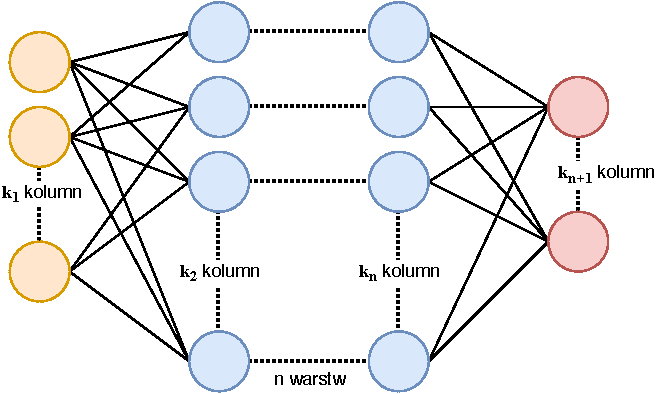
\includegraphics[scale=0.9]{resources/fc/fully_connected.pdf}}
\caption{Schemat w pełni połączonej sieci neuronowej.}
\label{fig:schematFc}
\end{figure}

W przypadku, gdy model zawiera stosunkowo dużą liczbę warstw ukrytych, na schemacie oznaczonych jako n, mówimy o głębokich sieciach neuronowych. 
Ten wariant sieci neuronowej charakteryzuje się tym, że każdy węzeł jej warstwy jest połączony z każdym. Warstwa wejściowa, oznaczona kolorem żółtym, doprowadza dane wejściowe do warstw ukrytych oznaczonych kolorem niebieskim. Warstwa wyjściowa oznaczona jest kolorem czerwonym.

\section{Neuron gęstej sieci neuronowej}
Pojedynczy neuron można przedstawić następującym schematem \ref{fig:neuronFc}.

\begin{figure}[ht]
\centerline{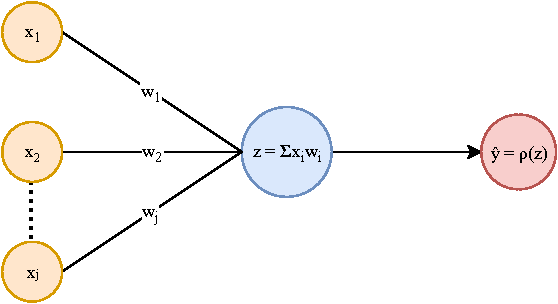
\includegraphics[scale=1]{resources/fc/single_neuron_fc.pdf}}
\caption{Schemat w pełni połączonej sieci neuronowej.}
\label{fig:neuronFc}
\end{figure}

Wartości \(a_1\) do \(a_j\) reprezentują wartości z warstwy sieci neuronowej, a w szczególności wartości początkowe \(x_1 ... x_j\). Każda z nich jest przemnożona przez odpowiadającą jej wagę \(w\) i zsumowana. Następnie, tak uzyskaną wartość używamy do wyliczenia \(\rho\) nazwanego funkcją aktywacji neuronu. Zadaniem \(\rho\) jest wprowadzenie elementu nieliniowości. Mniej formalnie, ma na celu ustalenie czy neuron powinien zostać aktywowany czy też nie.
Najpopularniejsze funkcje aktywacji przedstawia rysunek \ref{fig:activations}.

\begin{figure}
\subfloat[Funkcja \textit{ReLU}.]{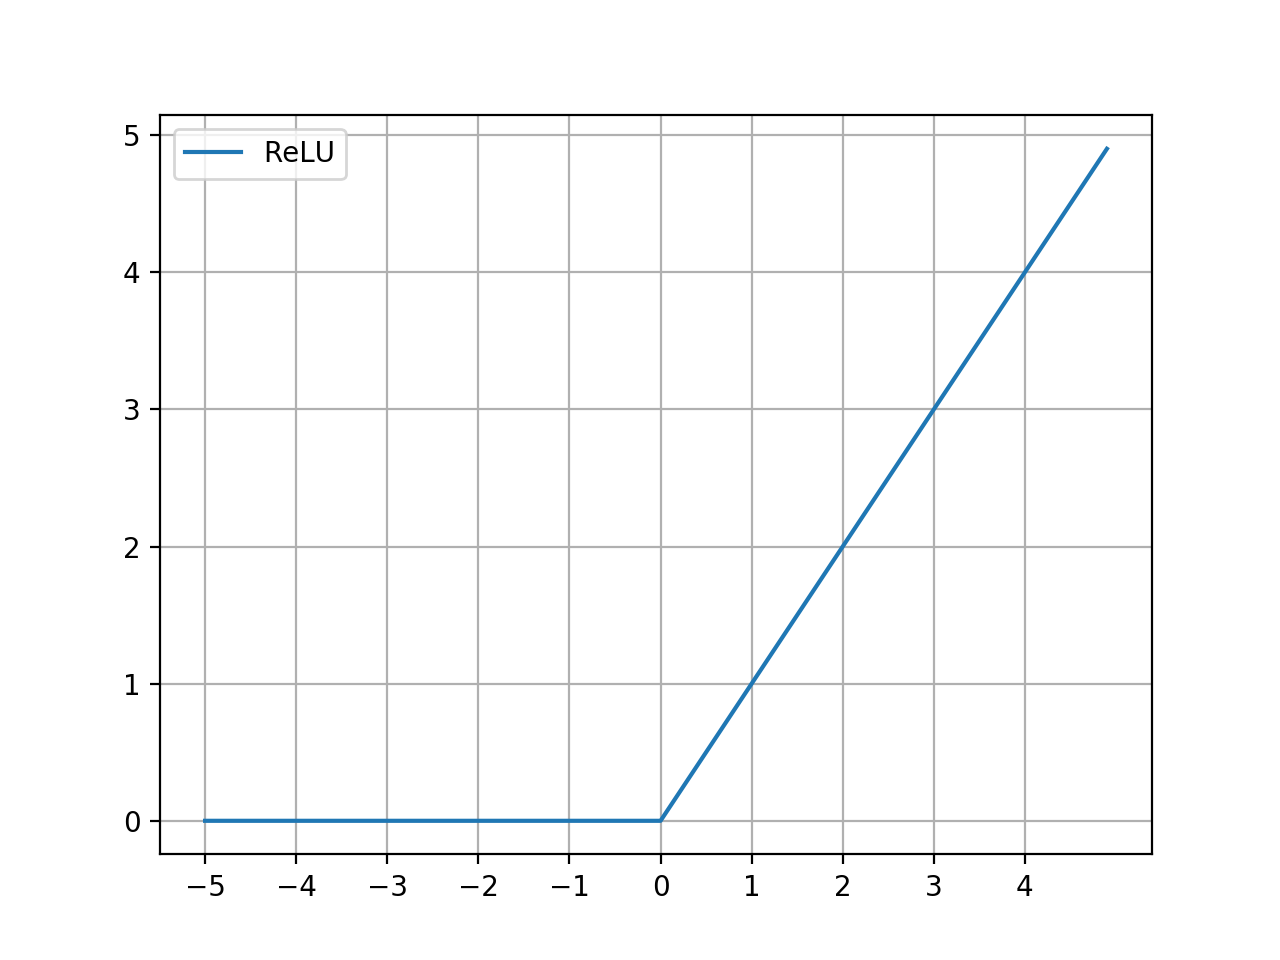
\includegraphics[width = 2in]{resources/fc/relu.png}} 
~
\subfloat[Funkcja \textit{Sigmoid}.]{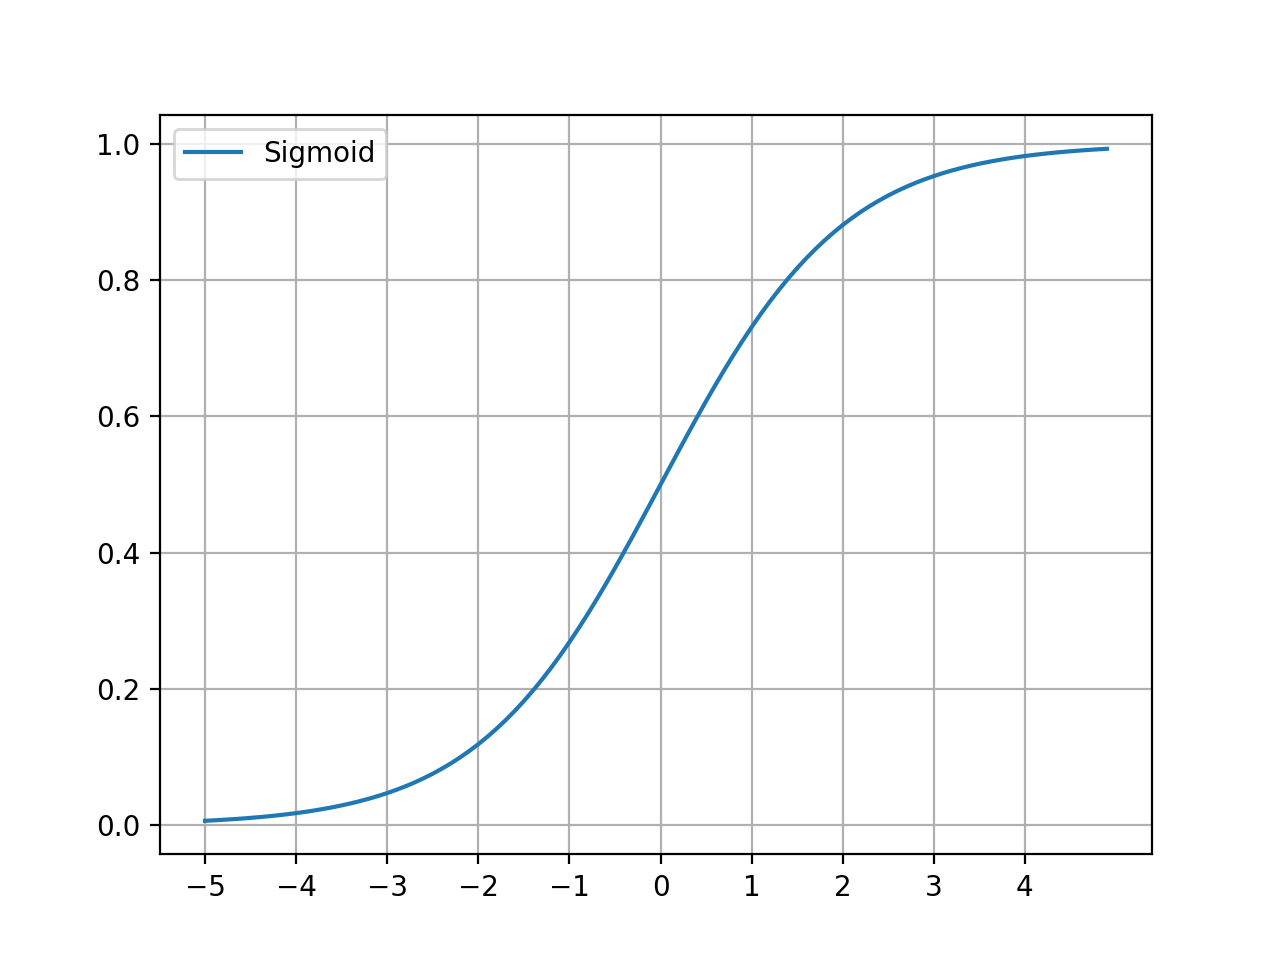
\includegraphics[width = 2in]{resources/fc/sigmoid.png}} 
~
\subfloat[Funkcja \textit{tangens hiperboliczny}.]{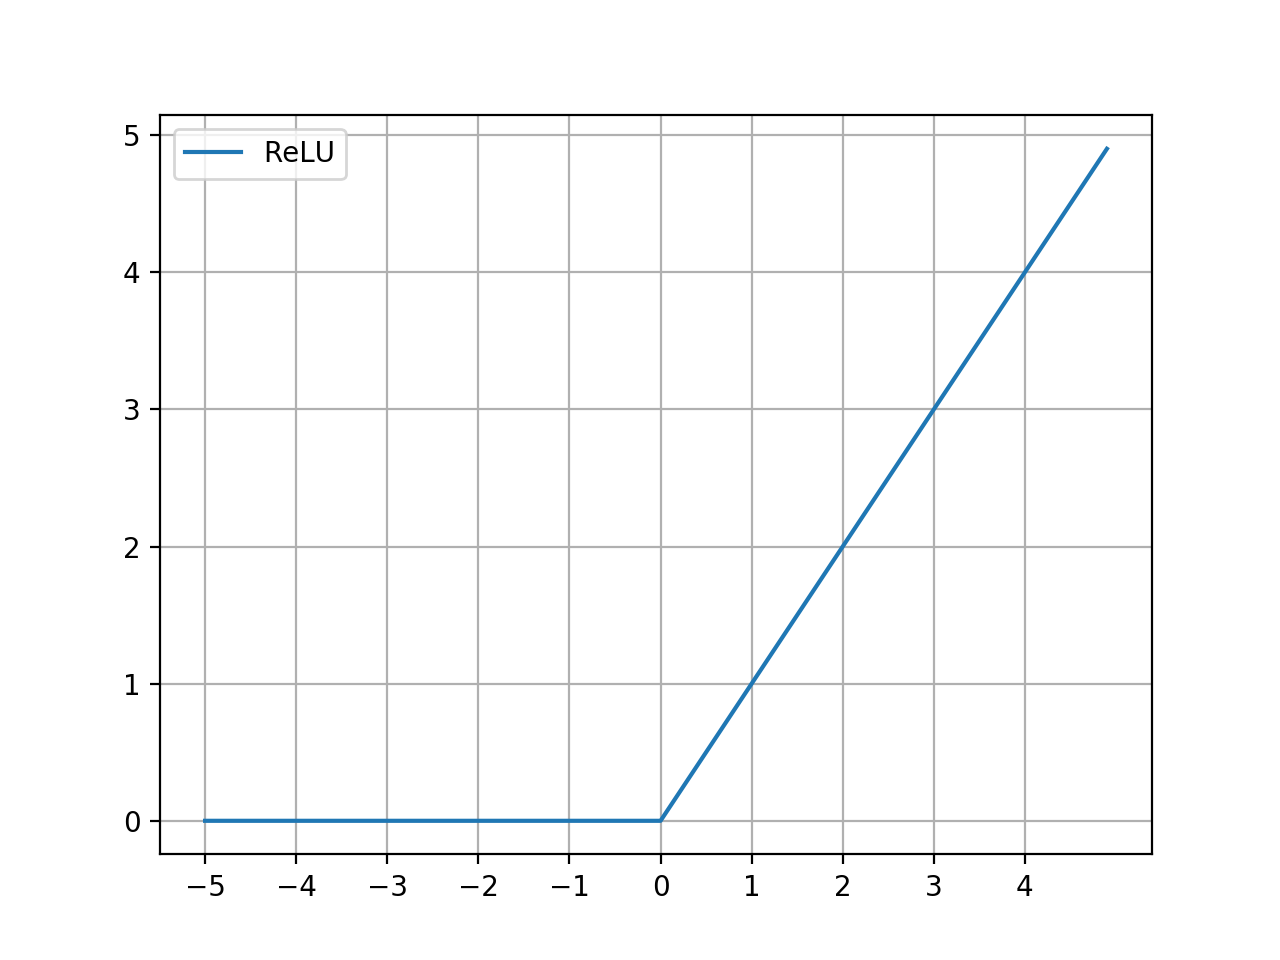
\includegraphics[width = 2in]{resources/fc/relu.png}} 
\caption{Wybrane funkcje aktywacji.}
\label{fig:activations}
\end{figure}

\section{Propagacja w przód}

By ustalić wartość neuronu, posługujemy się następującym wzorami:

\[z_{n}^{\lbrack l\rbrack}=\sum_{i=1}^{j}{w_{\text{ni}}^{\lbrack l\rbrack}a_{i}^{\lbrack l - 1\rbrack} + b_{n}^{\lbrack l\rbrack}},\]

\[a_{n}^{\lbrack l\rbrack}=\rho(z_{n}^{\lbrack l\rbrack}),\]

Gdzie:
\begin{itemize}
\item \(\rho\) to funkcja aktywacji,
\item \textsubscript{(n)} oznacza numer neuronu w warstwie,
\item \textsuperscript{{[}l{]}} to numer warstwy,
\item \(b\) to tak zwany bias. Jego wartość jest ustalana razem z wagami w procesie propagacji wstecznej,
\item \(w_{\text{ni}}^{\lbrack l\rbrack}\) jest to \textbf{i}-ta waga neuronu numer \textbf{n}, warstwy \textbf{l},
\item \(a_{i}^{\lbrack l - 1\rbrack}\) jest to wartość \textbf{i}-tego neuronu warstwy \({[}l-1{]}\), w szczególnym przypadku może być to jedna z wartości wejściowych \(x\).
\end{itemize}

Używając tych wzorów, możemy obliczać wartości wag kolejnych warstw sieci aż do warstwy ostatniej.
Tam, w zależności od postawionego problemu, możemy wyliczyć kolejne aktywacje przy pomocy \(\rho\) (tylko w odróżnieniu od warstw ukrytych nie stosuje się tam \(ReLU\), tylko np. \(sigmoid\) lub możemy użyć funkcji \(softmax\):

\[S(y_{i}) = \frac{e^{y_{\text{i\ }}}}{\sum_{j}^{y_{n}}e^{y_{j}}}\]

Jest to funkcja, która przyjmuje \(y_{n}\) elementowy wektor składający się z liczb rzeczywistych i przeprowadza go w rozkład prawdopodobieństwa składającego się z \(y_{n}\) elementów. Przydatną jej cechą jest to, że zachowuje proporcjonalny udział wartości w wynikowym prawdopodobieństwie -- tj. elementy o wyższej wartości mają przypisane wyższe wartości prawdopodobieństwa.

Na przykładzie klasyfikacji, by uzyskać wynik, który można zinterpretować, należy posłużyć się następującym sposobem postępowania. Niech przedostatnia warstwa \(a^{\lbrack L - 1\rbrack}\) sieci posiada \(n\) węzłów, których liczba jest równa liczbie klas rzeczy, które chcemy rozpoznawać. Przyjmijmy również, że dana rzecz nie może należeć do dwóch klas równocześnie.

W przypadku aktywacji przy pomocy sigmoid uzyskujemy algorytm nazywany ,,jeden kontra każdy'' (ang. \textit{one vs all}). Każdy z węzłów \(a_{i}^{\left\lbrack L - 1 \right\rbrack}\) jest wejściem dla \(\rho\). Po wyliczeniu wartości, przyjmujemy próg z przedziału \({[}0, 1{]}\), by uzyskać wynik dla każdego neuronu z osobna.

\begin{figure}[ht]
\centerline{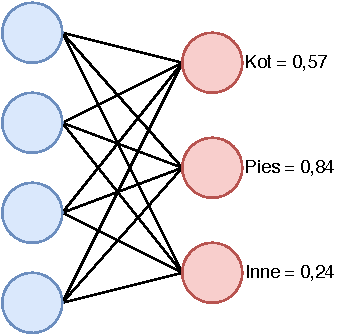
\includegraphics[scale=1]{resources/fc/sigmoid_1vsAll.pdf}}
\caption{Przykładowy wynik \textit{1 vs all} dla trzech klas ze zbioru \big\{Kot, Pies, Inne.\big\}}
\label{fig:1v_all}
\end{figure}

By zobrazować działanie algorytmu posłużę się przykładem. Załóżmy, że zbudowano klasyfikator, mający na celu przypisanie danej postaci klasy ze zbioru {kot, pies, inne}. Każdą aktywację z warstwy \(L-1\) przeprowadzamy z osobna, przy pomocy \(sigmoid\) w wartość z przedziału od 0 do 1. Następnie, przyjmujemy próg, powyżej którego mówimy, że sieć rozpoznała daną klasę. Przykładowo, w przypadku z rysunku \ref{fig:1v_all} przyjmując próg równy 0.5 mamy dwa możliwe wyniki. By wyeliminować jeden z nich możemy zwiększyć próg do 0.6 lub wybrać neuron z wyższą wartością. W obu przypadkach będzie to neuron oznaczający to, że klasyfikator rozpoznał psa.

\begin{figure}[ht]
\centerline{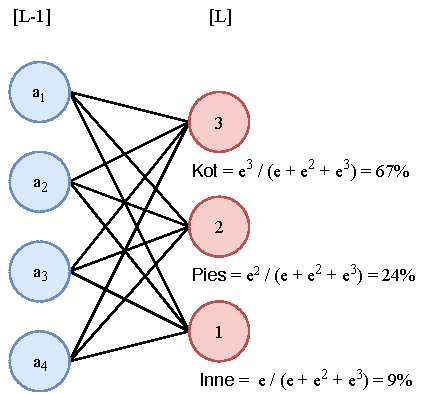
\includegraphics[scale=1]{resources/fc/softmax_fc.pdf}}
\caption{Przykładowy wynik z użyciem \textit{softmax}.}
\label{fig:softmax}
\end{figure}

Istnieją inne metody aktywacji warstw wyjściowych. Każda z nich, która zostanie użyta w tej pracy będzie trzymała się podobnego schematu. Wynikiem sieci gęsto połączonej będzie wektor zer i jedynek, w którym 1 ustawione na odpowiednim miejscu w rzędzie będzie oznaczało, że dany przedmiot został rozpoznany. W przypadku rozrysowanym na rysunku \ref{fig:softmax} będzie to wektor \([1 0 0]\).

\section{Funkcja kosztu}
\label{sec:costfunction}

W przypadku problemów poruszanych w tej pracy, funkcję kosztu należy rozumieć jako przyporządkowanie wynikom uzyskanym przy pomocy sieci neuronowej wraz ze znanymi poprawnymi odpowiedziami, liczby reprezentującej „koszt”. Wartość kosztu należy interpretować jako skuteczność w odgadywaniu poprawnych wyników w taki sposób, że im niższy koszt tym wyższa poprawność predykcji. Można powiedzieć, że sieć neuronowa próbuje znaleźć najwierniejsze przybliżenie oryginalnej, nieznanej funkcji nazywanej hipotezą, a celem funkcji kosztu jest modelowanie różnicy między przybliżeniem a funkcją, której próbujemy nauczyć sieć.

Istnieje wiele różnych funkcji kosztu. Opiszę tutaj tylko funkcję \textit{cross entropy loss}, która jest często wybierana przy treningu sieci, które na ostatniej warstwie używają \(softmax\).

\[J(w) = \frac{1}{m}\ \sum_{i = 1}^{m}{\lbrack y_{i}\log{\acute{y}_{i} + \left( 1 - y_{i} \right)\log{(1 - \ \acute{y}_{i})}}\rbrack},\]

gdzie:

\begin{itemize}
\item
  \(w\) -- wagi sieci neuronowej,
\item
  \(m\) -- liczba klasyfikowanych przykładów,
\item
  \(y_{i}\) -- wartość oczekiwana dla przykładu numer i
\item
    \(\acute{y}_{i}\) -- wartość uzyskana przy pomocy sieci dla przykładu numer \(i\).
\end{itemize}

Jest to suma błędów pojedynczych predykcji dla wszystkich przykładów dostępnych w danym zestawie danych treningowych. Zadaniem treningu, będzie znalezienie jej minimum dla danego problemu.
By udało się to sprawnie zrobić, będę korzystał z faktu, że ta i inne funkcje kosztu, którymi będę się posługiwał są różniczkowalne i ciągłe.

\section{Propagacja wstecz}
\label{sec:backprob}

Jest to modyfikacja wag sieci neuronowej \(w\) z uwzględnieniem funkcji kosztu \(J(w)\). Popularnym sposobem jest metoda gradientu prostego (częściej spotykana w wariacji z tzw. pędem, z angielskiego \textit{Gradient descent with momentum} lub dalsze jej modyfikacje jak np. algorytm
\textit{Adaptive moment estimation}, znany jako \textit{Adam}). W swej najprostszej wersji można sprowadzić go do następujących kroków:

\begin{enumerate}
\def\labelenumi{\arabic{enumi}.}
\item
  Wybierz punkt startowy \(w_{0}\).
\item
  \(w_{k + 1} = w_{k} - \alpha\ \nabla f(w_{k})\).
\item
  Jeżeli \(\left\| w_{k + 1} - w_{k} \right\|\  \geq \varepsilon\) idź
  do 2.
\item
  Koniec.
\end{enumerate}

gdzie:

\begin{itemize}
\item
  \(\alpha\) -- współczynnik uczenia: zazwyczaj niewielka
  (\(\alpha\  < 0.01)\) dodatnia liczba rzeczywista. Podczas treningu
  sieci neuronowych często \(\alpha = const\), choć sam algorytm
  gradientu prostego posiada wariację ze zmienną wartością \(\alpha\).
\item
  \(\nabla f(w_{k})\) -- jest to gradient funkcji reprezentującej
  funkcję przybliżającą hipotezę.
\item
  \(w\) -- wagi sieci,
\item
  \(\varepsilon\) -- niewielka wartość będąca kryterium stopu dla
  algorytmu. Wykorzystuje fakt, że różnice w wartości wag będą maleć
  wraz ze zbliżaniem się do minimum funkcji \(J(w)\).
\end{itemize}

Krok pierwszy, czyli wybranie punktu startowego jest rozwiązany przy pomocy losowej inicjalizacji wag \(w\). Często stosuje się tu różne heurystyki dostosowane do użytej funkcji aktywacji (dla \(\tanh\) jest to przykładowo inicjalizacja \(Xaviera\).

Kłopotliwym zagadnieniem może wydawać się wyliczenie gradientu \(\nabla f(w)\). Nie posiadając formalnej definicji hipotezy, tylko jej aproksymację w postaci sieci neuronowej musimy, posłużyć się funkcją kosztu \(J(w)\) i zależnością:

gdy:

\[J\left( z \right) = J(a\left( z \right))\]

to:

\[\frac{dJ}{dz} = \frac{dJ}{da} \frac{da}{dz}\]

Posługując się nimi, możemy wyjść od wzoru funkcji kosztu \(J(w)\) i na tej podstawie aktualizować wartość wag ostatniej warstwy. Co więcej, możemy przy pomocy nowo wyliczonych wag, wyliczyć nowe wartości wag warstwy przedostatniej i tak niejako licząc warstwa po warstwie, aktualizować wszystkie wagi sieci neuronowej.

Niestety konkretne wzory służące do aktualizacji wag muszą być wyprowadzone dla każdej z funkcji kosztu z osobna. Całe szczęście biblioteki do uczenia maszynowego mają zaimplementowane większość z nich w taki sposób, że użytkownik musi tylko zaimplementować propagację w przód i wybrać funkcję kosztu. Nie mniej jednak, by zobrazować ten proces wyprowadzę wzory potrzebne dla propagacji wstecznej dla dwuwarstwowej sieci neuronowej. Propagację na dalsze warstwy będą tylko ponownym wykorzystaniem
tych samych wzorów w zastosowaniu do kolejnych wag.

Schemat sieci neuronowej wykorzystanej do obliczeń znajduje się na rysunku \ref{fig:backprop_fc}.

\begin{figure}[ht]
\centerline{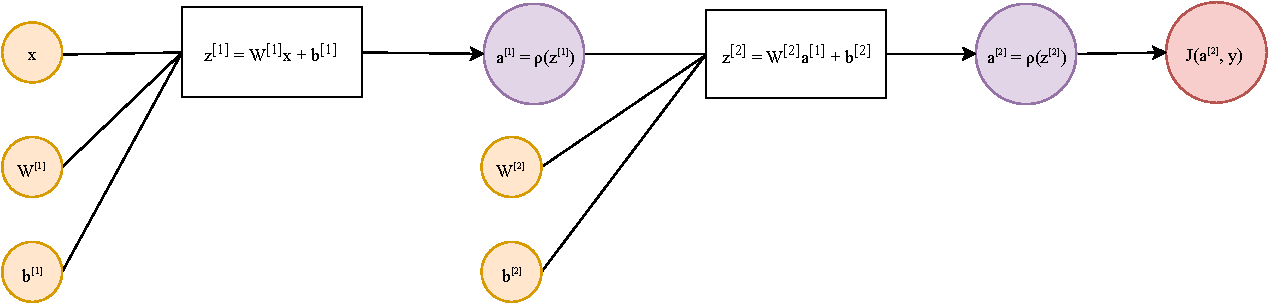
\includegraphics[scale=0.7]{resources/fc/backprop_fc_cross_entropy.pdf}}
\caption{Przykładowy schemat sieci neuronowej, przy liczeniu propagacji
wstecznej.}
\label{fig:backprop_fc}
\end{figure}

Dla pojedynczego przykładu ze zbioru treningowego:

\[J\left( w \right) = y\log{a(w)^{\lbrack 2\rbrack} + \left( 1 - y \right)\log{(1 - \ a(w)^{\lbrack 2\rbrack})}}\]

oraz przyjmując \(sigmoid\) za funkcję aktywacji:

\[\rho = \frac{e^{z}}{e^{z}\  + \ 1},\]

wtedy:

\begin{enumerate}
\def\labelenumi{\arabic{enumi}.}
\item
  \(\frac{dJ}{da^{\left\lbrack 2 \right\rbrack}} = - \frac{y}{a^{\lbrack 2\rbrack}} + \frac{1 - y}{1 - a^{\lbrack 2\rbrack}},\)
\item
    \(\frac{da^{\left\lbrack 2 \right\rbrack}}{dz^{\lbrack 2\rbrack}} = \frac{d\rho^{\lbrack 2\rbrack}}{dz} = \frac{e^{z^{\left\lbrack 2 \right\rbrack}}}{\left( 1\  + {\ e}^{z^{\left\lbrack 2 \right\rbrack}} \right)^{2}} = \frac{e^{-z^{\left\lbrack 2 \right\rbrack}}}{\left( 1\  + {\ e}^{-z^{\left\lbrack 2 \right\rbrack}} \right)^{2}} = \frac{1}{1\  + {\ e}^{- z^{\lbrack 2\rbrack}}} \frac{1\  + \ \left( e^{- z^{\left\lbrack 2 \right\rbrack}} \right)\ \  - \ 1}{\left( 1\  + {\ e}^{- z^{\left\lbrack 2 \right\rbrack}} \right)} = \frac{1}{1\  + {\ e}^{- z^{\left\lbrack 2 \right\rbrack}}} (1 - \frac{1}{\left( 1\  + {\ e}^{- z^{\left\lbrack 2 \right\rbrack}} \right)}) = a^{\lbrack 2\rbrack}(1 - a^{\left\lbrack 2 \right\rbrack})\),
\item
  \(\frac{dJ}{dz^{\left\lbrack 2 \right\rbrack}} = \frac{dJ}{da^{\left\lbrack 2 \right\rbrack}} \frac{da^{\left\lbrack 2 \right\rbrack}}
  {dz^{\left\lbrack 2 \right\rbrack}} = \left\lbrack - \frac{y}{a^{\left\lbrack 2 \right\rbrack}} + \frac{1 - y}{1 - a^{\left\lbrack 2 \right\rbrack}}
  \right\rbrack a^{\left\lbrack 2 \right\rbrack}\left( 1 - a^{\left\lbrack 2 \right\rbrack} \right) = - \left\lbrack \frac{y\left( 1 - a^{\lbrack 2\rbrack} \right)\  + \ a^{\lbrack 2\rbrack}
  \left( 1 - y \right)}{a^{\lbrack 2\rbrack}\left( 1\ -\ a^{\lbrack 2\rbrack} \right)} \right\rbrack a^{\left\lbrack 2 \right\rbrack}
  \left( 1 - a^{\left\lbrack 2 \right\rbrack} \right) = \ a^{\left\lbrack 2 \right\rbrack} - y\).
\end{enumerate}

Dysponując \(\frac{dJ}{dz^{\left\lbrack 2 \right\rbrack}}\),
\(a^{\lbrack 2\rbrack}\) i \(a^{\lbrack 1\rbrack}\) (z fazy propagacji
w przód) możemy zaktualizować \(w^{\lbrack 2\rbrack}\) i
\(b^{\lbrack 2\rbrack}\),

\begin{enumerate}
\def\labelenumi{\arabic{enumi}.}
\setcounter{enumi}{3}
\item
  \(\frac{dJ}{dw^{\lbrack 2\rbrack}} = \frac{dJ}{dz^{\left\lbrack 2 \right\rbrack}} \frac{dz^{\left\lbrack 2 \right\rbrack}}{dw^{\left\lbrack 2 \right\rbrack}} = {(a}^{\left\lbrack 2 \right\rbrack} - y)a^{\lbrack 1\rbrack}\),
\item
  \(\frac{dJ}{db^{\lbrack 2\rbrack}} = \ \frac{dJ}{dz^{\left\lbrack 2 \right\rbrack}} \frac{dz^{\left\lbrack 2 \right\rbrack}}{db^{\left\lbrack 2 \right\rbrack}} = \ {(a}^{\left\lbrack 2 \right\rbrack} - y)\).
\end{enumerate}

Powyższe obliczenia pokazują, w jaki sposób obliczyć nową wartość wag między funkcją kosztu a ostatnią warstwą sieci. Kolejne kroki pokażą, w jaki sposób obliczyć nową wartość wag pomiędzy dwiema warstwami (można te kroki uogólniać na dowolną liczbę warstw).

\begin{enumerate}
\def\labelenumi{\arabic{enumi}.}
\setcounter{enumi}{5}
\item
  \(\frac{dJ}{da^{\lbrack 1\rbrack}} = \frac{dJ}{dz^{\lbrack 2\rbrack}} \frac{dz^{\left\lbrack 2 \right\rbrack}}{da^{\left\lbrack 1 \right\rbrack}} = {(a}^{\left\lbrack 2 \right\rbrack} - y) w^{\lbrack 2\rbrack},\)
\item
  \(\frac{dJ}{dz^{\left\lbrack 1 \right\rbrack}} = \frac{dJ}{da^{\left\lbrack 1 \right\rbrack}} \frac{da^{\left\lbrack 1 \right\rbrack}}{dz^{\left\lbrack 1 \right\rbrack}} = {w^{\left\lbrack 2 \right\rbrack}(a}^{\left\lbrack 2 \right\rbrack} - y){a}^{\left\lbrack 1 \right\rbrack}(1 - a^{\left\lbrack 1 \right\rbrack}).\)
\end{enumerate}

(\(\frac{da^{\left\lbrack 1 \right\rbrack}}{dz^{\left\lbrack 1 \right\rbrack}}\)
obliczone analogicznie jak w kroku numer. 2),

Stąd wiadomo jak obliczyć wagi \(w^{\left\lbrack 1 \right\rbrack}\ \)i
\(b^{\left\lbrack 1 \right\rbrack},\)

\begin{enumerate}
\def\labelenumi{\arabic{enumi}.}
\setcounter{enumi}{7}
\item
  \(\frac{dJ}{dw^{\lbrack 1\rbrack}} = \frac{dJ}{dz^{\lbrack 1\rbrack}} \frac{dz^{\left\lbrack 1 \right\rbrack}}{dw^{\left\lbrack 1 \right\rbrack}} = {w^{\left\lbrack 2 \right\rbrack}(a}^{\left\lbrack 2 \right\rbrack} - y){a}^{\left\lbrack 1 \right\rbrack}(1 - a^{\left\lbrack 1 \right\rbrack}) x,\)
\item
  \(\frac{dJ}{db^{\lbrack 1\rbrack}} = \frac{dJ}{dz^{\lbrack 1\rbrack}} \frac{dz^{\left\lbrack 1 \right\rbrack}}{dw^{\left\lbrack 1 \right\rbrack}} = {w^{\left\lbrack 2 \right\rbrack}(a}^{\left\lbrack 2 \right\rbrack} - y){a}^{\left\lbrack 1 \right\rbrack}(1 - a^{\left\lbrack 1 \right\rbrack}).\)
\end{enumerate}

Po takim cyklu, należy wybrać kolejny przykład z zestawu treningowego, przeliczyć propagację w przód, funkcję kosztu a następnie znów propagację w tył, aż kryterium stabilności metody gradientu prostego zostanie spełnione.


\chapter{Neuronowa sieć konwolucyjna}
\label{chap:cnn}
\section{Wstęp}
\label{cnn-wstęp}
W przypadku zagadnień z dziedziny analizy obrazu, same sieci gęste robią się niepraktyczne. Teoretycznie możliwe jest przetworzenie obrazu w taki sposób, że każdy piksel traktowany jest jako jeden węzeł sieci, ale to już przy obrazkach o wymiarach 100x100x3 (100 na 100 pikseli, 3 kanały RGB) daje 30000 węzłów na warstwie pierwszej. Nawet gdyby warstwa druga
miała być dwa razy mniejsza tj. 15000 węzłów macierz \(w^{\lbrack 1\rbrack}\) miałaby wymiar (30000, 15000) przy założeniu, że rozmiar liczby typu double to 64 bity to sama taka pojedyncza macierz ważyłaby \(64\ \left\lbrack B \right\rbrack \bullet 30000 \bullet 15000 \bullet \frac{1}{8\ }\ \left\lbrack b \right\rbrack \bullet \frac{1}{1024\ }\left\lbrack \text{kb} \right\rbrack\frac{1}{1024\ }\left\lbrack \text{mb} \right\rbrack\  \approx \ 3422\ \lbrack mb\rbrack\). Poza problemami z pamięcią,
leży wziąć pod uwagę wysoki koszt obliczeniowy operacji na tak dużych macierzach, a przecież rozdzielczość współczesnych obrazów jest wielokrotnie wyższa. By poradzić sobie z tym problemem, należało wprowadzić inny rodzaj architektury sieci neuronowej -- konwolucyjną sieć neuronową.

\section{Opis elementów składających się na CNN}
\label{opis-elementów-cnn}

\subsection{Filtry i splot w CNN}

By ograniczyć ilość węzłów definiuje się tzw. filtry. Są to macierze kwadratowe wypełnione wagami \(w\) których wartość jest ustalana w procesie propagacji wstecznej. By uzyskać wynik, stosuje się na obrazie dyskretną operację splotu z zadanym \emph{krokiem} i \emph{dopełnieniem}.

\begin{figure}[ht]
\centerline{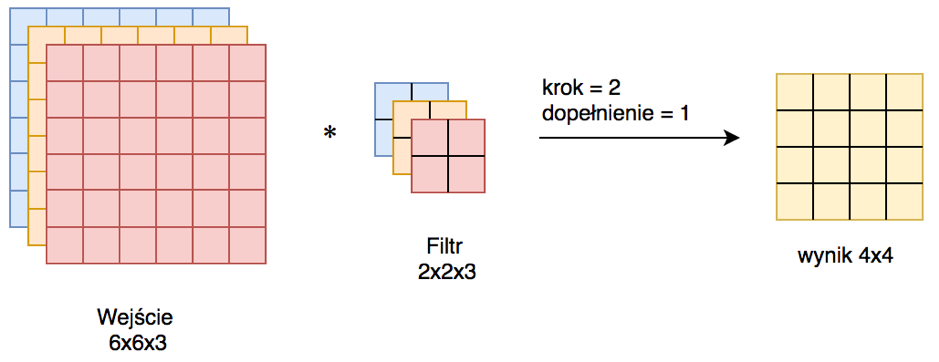
\includegraphics[scale=0.8]{resources/splot.png}}
\caption{Przykładowa operacja splotu wykonywana między dwiema warstwami sieci CNN.}
\label{fig:splot}
\end{figure}

Operację wykonaną pomiędzy pojedynczą warstwą wejściową a odpowiadającym jej filtrem można zapisać:

Niech: \(k = \left\lfloor \frac{n + 2p}{s} \right\rfloor\), \(k\ \in Z\)

\[\sum_{q = 0}^{n_{w}}{\sum_{p = 0}^{k}{\sum_{i = 0}^{n_{g} - 1}{\sum_{j = 0}^{n_{g} - 1}{\sigma\lbrack f_{q}\left( ps + i,ps + j \right) \bullet g_{q}\left( i,j \right) + b\rbrack}}}}\]

gdzie:

\begin{itemize}
\item
  \(n_{w}\) -- wielkość trzeciego wymiaru wejściowej macierzy,
\item
  n -- wymiar wejściowej macierzy kwadratowej, w tym przypadku równy 6,
\item
  p -- dopełnienie, wymiar dodatkowej „obwódki'' wokół oryginalnego
  obrazu w celu wyeliminowania tzw. problemu brzegu; w tym przypadku
  równe 1.
\item
  s -- krok, z którym dopasowujemy filtr na macierz wejściową, w tym
  wypadku równy 2, to znaczy macierz filtra jest aplikowana co dwa
  elementy w pionie i poziomie (każdy piksel jest zakryty wyłącznie
  raz),
\item
  \(n_{g}\)- wymiar macierzy filtra,
\item
  \(f_{q}(i,j)\) -- funkcja reprezentująca wartości macierzy wejściowej
  warstwy \(q\),
\item
  \(g_{q}(i,j)\) -- funkcja reprezentująca wartości macierzy filtra
  warstwy \(q\),
\item
  \(\sigma\) - funkcja aktywacji,
\item
  \(b\) -- bias.
\end{itemize}

Wzór zaproponowany powyżej jest analogicznym do gęstego modelu wzoru na
propagację wprzód \(z^{\lbrack l\rbrack} = w^{\lbrack l\rbrack}a^{\lbrack l - 1\rbrack} + b^{\lbrack l\rbrack},\ \ a^{\lbrack l\rbrack} = \sigma(z_{n}^{\lbrack l\rbrack})\). Jeżeli traktować \(w\), \(a\) i \(b\) jak macierze, a \(\sigma\) jako operację działającą na każdym z elementów macierzy z osobna.

Uzyskane tym sposobem macierze wynikowe oraz wagowe są wielokrotnie mniejsze, kosztem tego, że te same wagi są ustalane przy pomocy różnych części obrazu. Można za to wprowadzić wiele różnych zestawów filtrów. Każdy z nich, może nauczyć się wykrywać inne zależności w obrazie np. jeden może odpowiadać za wykrywanie krawędzi w pionie, inny w poziomie. W tym wypadku każdy z tych filtrów miałby wymiary 2\(\times\)2\(\times\)3. Stosując wiele różnych filtrów na raz uzyskujemy wielowymiarowy wynik,
wymiar trójwymiarowej macierzy wynikowej wynosi wtedy:
\[n_{x} \times n_{y} \times n_{z}\]
Gdzie \(n_{x}\) = ­­\(n_{y}\)=
\(\left\lfloor \frac{n + 2p - n_{f}}{s} \right\rfloor\), \(n,\ p,\ s\)
są zgodne z opisem wyżej, \(n_{f}\ \)to wymiar macierzy kwadratowej
filtra a \(n_{z}\) -- to ilość użytych filtrów wielkości
\(n_{f} \times n_{f} \times n_{z}\).

Należy jednocześnie nadmienić, że filtry nie muszą być stosowane tylko na danych wejściowych. Wynik konwolucji może i często jest, przekazywany do głębszych warstw, gdzie uczone są filtry pracujące na wynikach warstw poprzednich. O wizualizacji tego czego się te filtry nauczyły, będzie dalej w tej pracy.

\subsection{Warstwy łączące}

Warstwy łączące (ang. "pooling layers") są często wykorzystywane w celu zmniejszania wymiarów warstwy sieci CNN. Do najpopularniejszej należy zdecydowanie tzw. max pooling. Polega na tym, że z obszaru w macierzy reprezentującej wartości danej warstwy w sieci konwolucyjnej wybieramy element z najwyższą wartością.

\begin{figure}[ht]
\centerline{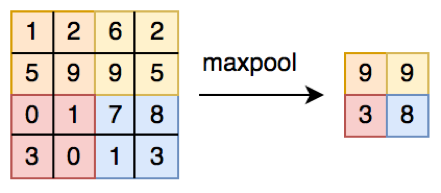
\includegraphics[scale=1]{resources/maxpool.png}}
\caption{Zasada działania maxpool dla macierzy 4x4 przy użycia filtra 2x2, bez dopełnienia i z krokiem s = 2.}
\label{fig:maxpool}
\end{figure}

Istnieje jeszcze wariacja sumująca wszystkie wartości z obszaru (ang. „sum pooling'') i licząca średnią z obszaru (ang. „avg pooling''). Zasady odnośnie liczenia wielkości macierzy wynikowej dotyczącą każdego z wariantów poolingu i są analogiczne jak w przypadku obliczania splotu, z tym wyjątkiem, że pooling stosowany jest do każdej z warstw osobno i nie wpływa na wielkość trzeciego wymiaru macierzy wynikowej.

Popularnym schematem jest ustawienia warstwy poolingowej zaraz po warstwie konwolucyjnej (wraz z wykonaniem aktywacji na wyniku). Warstwy splot-pooling często są łączone ze sobą w różnych wariantach architektury sieci CNN.

\section{Przykład sieci konwolucyjnej - LeNet-5}
\label{lenet5}

\subsection{Schemat sieci LeNet-5}

Przy użyciu splotu, warstw łączących i sieci gęsto połączonych, można zaprezentować kompletny model sieci konwolucyjnej. Posłużę się przykładem klasycznej sieci nazwanej LeNet-5. Oryginalnie służyła do rozpoznawania odręcznie pisanego pisma.

\begin{figure}[ht]
\centerline{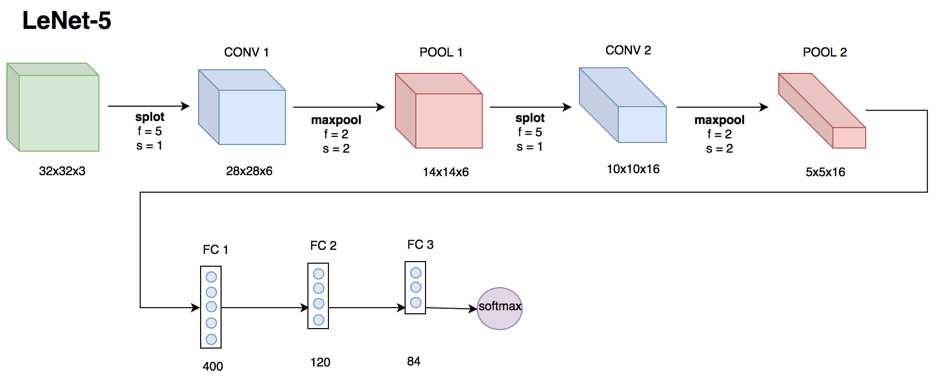
\includegraphics[scale=1]{resources/lenet5.png}}
\caption{Schemat sieci konwolucyjnej LeNet-5}
\label{fig:lenet5}
\end{figure}

Przyjmuje ona wejściu obrazki o wymiarach 32\(\times\)32 pikseli z trzema kanałami (RGB), stosuje operacje splotu przy użyciu 6 filtrów o wymiarach 5\(\times\)5\(\times\)3 dając, zgodnie ze wzorem, wynik o wymiarach 28\(\times\)28\(\times\)6. Do tak uzyskanych macierzy wprowadzany jest element nieliniowości przy pomocy funkcji aktywacji, w tym przypadku tangens hiperboliczny. Następnie stosowana jest warstwa maxpool o wymiarze filtra 2\(\times\)2\(\times\)6. Tak uzyskany wynik, trafia na splot
tym razem 16 filtrów 5\(\times\)5\(\times\)6 i maxpool 2\(\times\)2\(\times\)16. Następnie przekazywany jest do w pełni połączonej sieci neuronowej, trójwarstwowej, posiadającej 400, 120 i 84 węzły na kolejnych warstwach. W wersji, którą chce zaprezentować wynik uzyskam przy pomocy softmax i będzie to 10 elementowy wektor.

\subsection{Implementacja sieci LeNet-5}

By zaimplementować zaproponowany model, posłużę się biblioteką do
głębokiego uczenia maszynowego -- Keras. Model będzie zaimplementowany w
języku Python (wersja 3). Sieć będzie trenowana przy pomocy CPU. Do
treningu użyję publicznie dostępnej bazy danych mnist
(http://yann.lecun.com/exdb/mnist/). Dane zostaną podzielone w
sposób jaki został zaproponowany przez autorów tj. 60~000 przykładów
będzie użytych do treningu sieci a 10~000 do ewaluacji sprawności sieci.
Często pracuje się na trzech zbiorach danych: do uczenia, do regulacji
parametrów oraz do testów. W tym wypadku architektura sieci nie będzie
jednak zmieniana w trakcie treningu więc zestaw służący do regulacji
zostanie pominięty.

Dane dostępne w postaci binarnej zostaną wczytane na raz do pamięci RAM.
Następnie wartości pikseli obrazu zostaną znormalizowane z przedziału
{[}0, 255{]} do {[}0, 1{]}. Etykiety początkowo wczytywane są jako cyfra
z przedziału {[}0, 9{]}, w przypadku użycia softmax, istnieje potrzeba
dostosowania ich do postaci wektora składającego się z zer i jedynek w
którym, jedynka wstawiona na odpowiedniej pozycji pokazuje jaka jest
wartość etykiety (ang. „onehot vector'').

Niestety dostępne obrazy nie pasują formatem do zaproponowanej
oryginalnie sieci LeNet-5. Zamiast posiadać trzy kanały, obrazy
wejściowe są czarno białe i w wymiarach 28\(\times\)28 pikseli, więc
filtry pierwszej warstwy konwolucyjnej będą miały odpowiednio
zredukowany trzeci wymiar. By nie zmieniać zbytnio oryginalnej
architektury, obrazy zostały dopełnione przy pomocy zer na brzegach do
wymiaru 32\(\times\)32.

Sieć trenowana jest przy pomocy wariacji metody gradientu -- adam, użyta
funkcja kosztu to opisana w tej pracy „cross entropy loss''. Gdy sieć
jest trenowana przy pomocy adam, dane użyte do treningu grupowane są w
mniejsze porcje (w tym przypadku 256 elementów), na których przeliczana
jest propagacja wprzód i w tył na raz. Następnie, na sieci wynikowej
uczona jest następna porcja, aż do wyczerpania elementów ze zbioru
uczącego. Taki jeden obieg nazywamy epochem. Podczas treningu tej sieci
wykonam 5 takich epochów,

W celu uzyskania lepszej sprawności w przewidywaniach sieci,
zastosowałem w implementacji, nie opisane do tej pory praktyki
zapobiegające przeuczeniu sieci tzw. „dropout'' i normalizację porcji
(ang. „batch normalization''). Dropout, losowo „wyłącza'' poszczególne
neurony podczas uczenia, wymuszając równomierne rozłożenie
odpowiedzialności za wykrywanie poszczególnych cech zbioru danych. Batch
normalzation, natomiast skaluje wagi warstw ukrytych tak by mediana i
odchylenie standardowe nie zmieniały się zbyt drastycznie. Daje to
pozytywne efekty dla czasu treningu sieci i w pewnym stopniu, tak samo
jak dropout, normalizuje wagi
sieci.

\subsection{Implementacja modelu przy pomocy Keras}

Ten niewielki model, jest idealnym przykładem w jaki sposób modeluje się sieci neuronowe przy pomocy Kerasa. 
Kod do wczytywania danych został pominięty, ponieważ nie jest istotny z punktu widzenia treningu. 
Po wczytaniu danych, obrazy użyte do treningu są dopełniane do wielkości 32\(\times\)32 przy pomocy metody ZeroPadding2D, 
następnie przy pomocy Conv2D definiuje warstwę konwolucyjną, normalizuję jej wagi przy pomocy BatchNormalization i 
aktywuję przy pomocy tangensa hiperbolicznego. Następnie, stosuję warstwę MaxPooling2D, analogiczne warstwy 
Conv2D oraz BatchNormalization i całość wprowadzam do warstw gęstej sieci (warstwy Dense), stosując uprzednio dwa razy Dropout.

\label{lst:lenet5keras}
\begin{lstlisting}[language=Python, caption={Model sieci LeNet-5 w Keras.}, captionpos=b]
#loading the dataset
train_labels, test_labels, train_images, test_images, 
              train_images_orig, test_images_orig = loadTrainingData();
## model fitting below ##
X_input = Input((28, 28, 1))
# Padding to the 32x32
X = ZeroPadding2D((4, 4))(X_input)
# CONV -> BN -> RELU
X = Conv2D(6, (5, 5), strides = (1, 1), name = 'conv0')(X)
X = BatchNormalization(axis = 3, name = 'bn0')(X)
X = Activation('tanh')(X)
# MAXPOOL
X = MaxPooling2D((2, 2), name='max_pool_1', strides=2)(X)
# CONV -> BN -> RELU
X = Conv2D(16, (5, 5), strides = (1, 1), name = 'conv1')(X)
X = BatchNormalization(axis = 3, name = 'bn1')(X)
X = Dropout(0.4, name='drop_1')(X)
X = Dropout(0.3, name="drop_2")(X)
X = Dense(400, activation='tanh', name='fc_in')(X)
X = Dense(120, activation='tanh', name='fc_mid')(X)
X = Dense(84, activation='tanh', name='fc_out')(X)
X = Dense(10, activation='softmax', name='fc_softmax')(X)
# Create model
model = Model(inputs = X_input, outputs = X, name='ResNet-5')
model.compile(optimizer="Adam", 
              loss="binary_crossentropy", metrics=["accuracy"])
# Fit the model
model.fit(x=train_images, y=train_labels, epochs=5, batch_size=256)
# Evaluate
preds = model.evaluate(x = test_images, y = test_labels)
print ("Loss = " + str(preds[0]))
print ("Test Accuracy = " + str(preds[1]))
\end{lstlisting}

Model zdefiniowany przy pomocy klasy Model, trenowany jest przy pomocy funkcji optymalizującej Adam przy użyciu funkcji 
kosztu „binary crossentropy'' zdefiniowanych przy pomocy metody compile. Trening modelu zaczyna się po wywołaniu metody fit, przyjmującej dane na których ma być wtrenowana.
Metoda evaluate testuje skuteczność modelu na danych testowych.

\begin{figure}[ht]
\centerline{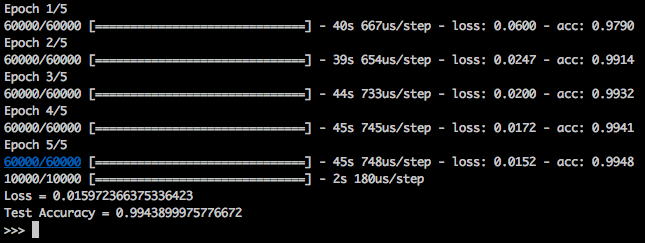
\includegraphics[scale=0.5]{resources/training_lenet5.png}}
\caption{Wynik treningu sieci LeNet-5.}
\label{fig:lenet5-training}
\end{figure}

Trening trwał niecałe 4 minuty i uzyskał skuteczność powyżej 99\% co jest bardzo zadawalającym wynikiem.

\begin{figure}[ht]
\centerline{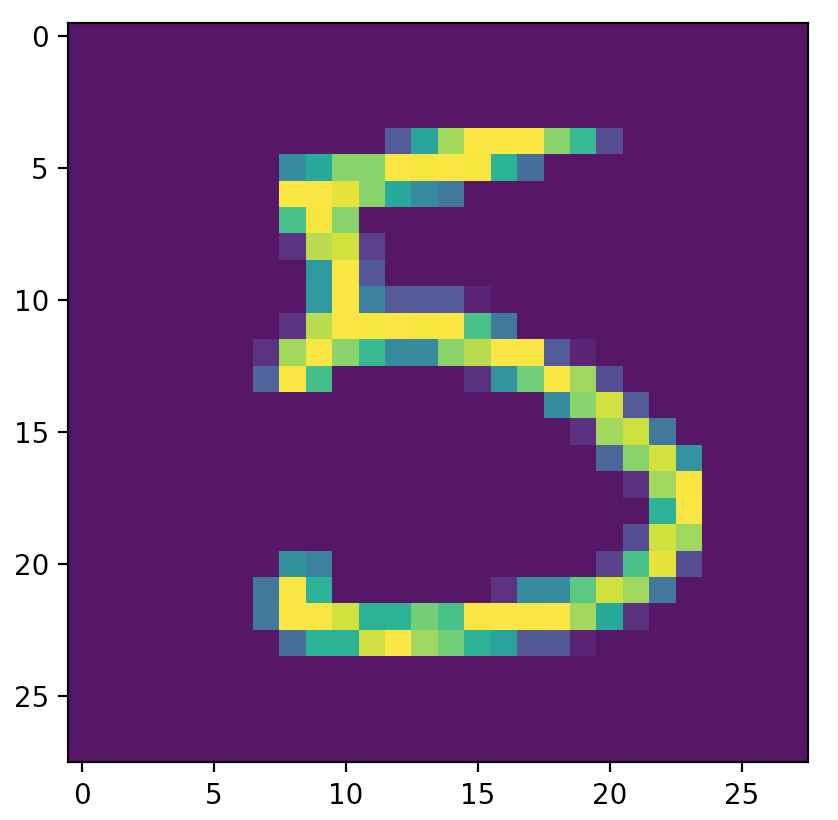
\includegraphics[scale=0.5]{resources/example_digit_lenet5.png}}
\caption{Przykładowy obraz ze zbioru testowego.}
\label{fig:lenet5-digit}
\end{figure}

\begin{figure}[ht]
\centerline{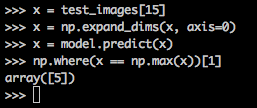
\includegraphics[scale=0.5]{resources/example_digit_lenet5_response.png}}
\caption{Odpowiedź modelu na pytanie, jaką cyfrę rozpoznaje.}
\label{fig:lenet5-response}
\end{figure}

\subsection{Wizualizacja neuronów warstw konwolucyjnych sieci LeNet-5.}
Mając do dyspozycji wytrenowany model, można przystąpić do próby wizualizacji tego czego nauczyła się sieć. Przy modelu tak płytkim jak LeNet-5 uzyskane odpowiedzi powinny być mniej imponujące wizualnie, ale przez to łatwiejsze w interpretacji.

\subsubsection{Wizualizacja poprzez wyświetlenie wag warstw konwolucyjnych.}
Pierwszy ze sposobów, który zaprezentuję będzie też najprostszy koncepcyjnie. Wyrysowanie filtrów warstw konwolucyjnych powinno dać ogólny zarys tego, jakie cechy obrazu (gradient, linie poziome/pionowe/ukośne) były brane pod uwagę przez sieć. W celu łatwiejszej intrepretacji zestawię ze sobą filtry 5\(\times\)5 oryginalnie występujące w sieci LeNet-5 z wariacją sieci wytrenowanej na filtrach 3\(\times\)3, którą wytrenowałem tylko po to by mieć punkt odniesienia do filtrów
klasycznie używanych w analizie obrazu.

\begin{figure}[ht]
\centerline{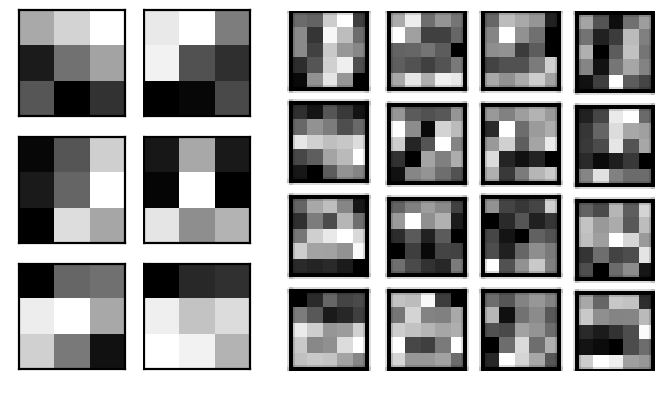
\includegraphics[scale=0.5]{resources/plot_filtry.png}}
\caption{Wizualizacja filtrów sieci LeNet-5. Od lewej filtry warstwy pierwszej wersji zmodyfikowanej 3\(\times\)3. Z prawej filtry warstwy drugiej wersji oryginalnej.}
\label{fig:lenet5-response}
\end{figure}

Na filtrach 3\(\times\)3 widać mocną tendencję w wykrywaniu krawędzi pionowych, poziomych i ukośnych. Dodatkowo duży nacisk położony jest na wykrywanie gradientu po skosie (dwa pierwsze filtry od góry i dwa ostatnie od dołu).

W przypadku filtrów 5\(\times\)5 kształty, które próbuje dopasować sieć robią się bardziej skomplikowane, przez co trudniejsze w interpretacji. Podobnie jak w przypadku filtrów warstwy pierwszej można znaleźć filtry szukające ukośnych gradientów oraz linii w pionie i poziomie, ale oprócz tego znajdują się tu filtry, które intrepretowałbym jako elementy strukturalne próbujące dopasować się do konkretnych kształtów występujących w poszczególnych elementach. Należy jednak podkreślić, że
wyświetlone filtry 5\(\times\)5 operują na wyniku konwolucji i maxpoolingu warstwy pierwszej -- są przez to ciężkie w intrepretacji.

Wniosek jest taki, że tym wypadku najprostsze rozwiązanie nie jest najlepsze. Nie będę więc dalej analizował tej metody ani stosował jej dla modeli o większej złożoności bo im głębszą warstwę sieci wybiorę tym trudniejsze w intrepretacji będą wyniki.

\subsubsection{Wizualizacja poprzez mapy cech.}
Mapy cech czy inaczej mapy aktywacji, wizualizują rezultat zastosowania filtrów na danych wejściowych -- np. obrazu wejściowego czy innej mapy cech. Przykładowo, dla danego obrazu można wyrysować jakie konkretnie jego cechy zostały wyszczególnione przez warstwę sieci CNN. 
By uzyskać mapę cech dla danego obrazu, należy zmodyfikować model w taki sposób by jego warstwą wyjściową była ta warstwa konwolucyjna, której cechy chcemy uzyskać

\label{lst:lenet5keras-mapy}
\begin{lstlisting}[language=Python, caption={Uzyskiwanie mapy aktywacji dla danego modelu i obrazu w Keras.}, captionpos=b]
img = np.expand_dims(img, axis=0)
vmodel = Model(inputs=model.inputs, outputs=model.layers[layer_no].output)
feature_maps = vmodel.predict(img)
\end{lstlisting}

W ogólności, warstwy bliżej źródła danych powinny zawierać informacje o dużej ilości szczegółów, a warstwy głębsze, wykrywać cechy bardziej ogólne. I tak, 
dla pierwszej warstwy konwolucyjnej sieci LeNet-5 wyrysowane cechy dla przykładu z każdej klas bardzo mocno przypominają oryginalne obrazy. Dostrzegalne różnice pomiędzy warstwami polegają na dostrzeganiu innego ''konturu'' obrazu, każda z warstw akcentuje inny jego rodzaj, przez co liczby dają iluzję bycia ''oświetlonymi'' z różnych stron.
Zgadza się to z obserwacją poczynioną w przypadku analizy wartości filtrów. Obraz niejako skanowany jest z każdej strony a uzyskany gradient determinuje z jaką klasą mamy do czynienia.

\begin{figure}[ht]
\centerline{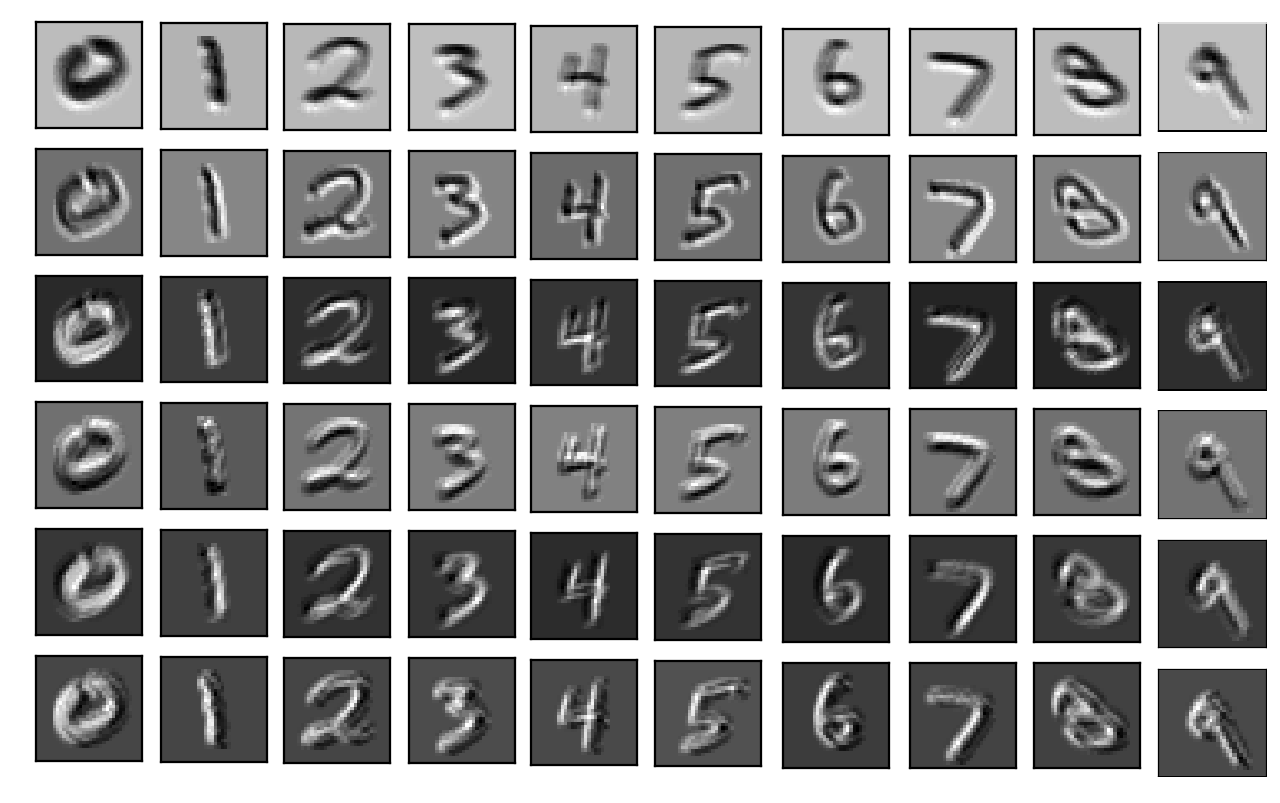
\includegraphics[scale=0.25]{resources/first_layer_gd_lenet.png}}
\caption{Mapy aktywacji dla 6 filtrów warstwy pierwszej, przy użyciu przykładu dla każdej z klas.}
\label{fig:lenet5-mapy-aktywacji-l1}
\end{figure}

Sytuacja robi się jeszcze ciekawsza w przypadku warstwy drugiej. Tam jest już 16 filtrów, więc nie zostaną zaprezentowane dla każdej z klas z osobna. Niemniej jednak, sam wynik dla pojdynczej klasy jest w stanie wiele powiedzieć na temat branych pod uwagę cech.

\begin{figure}[ht]
\centerline{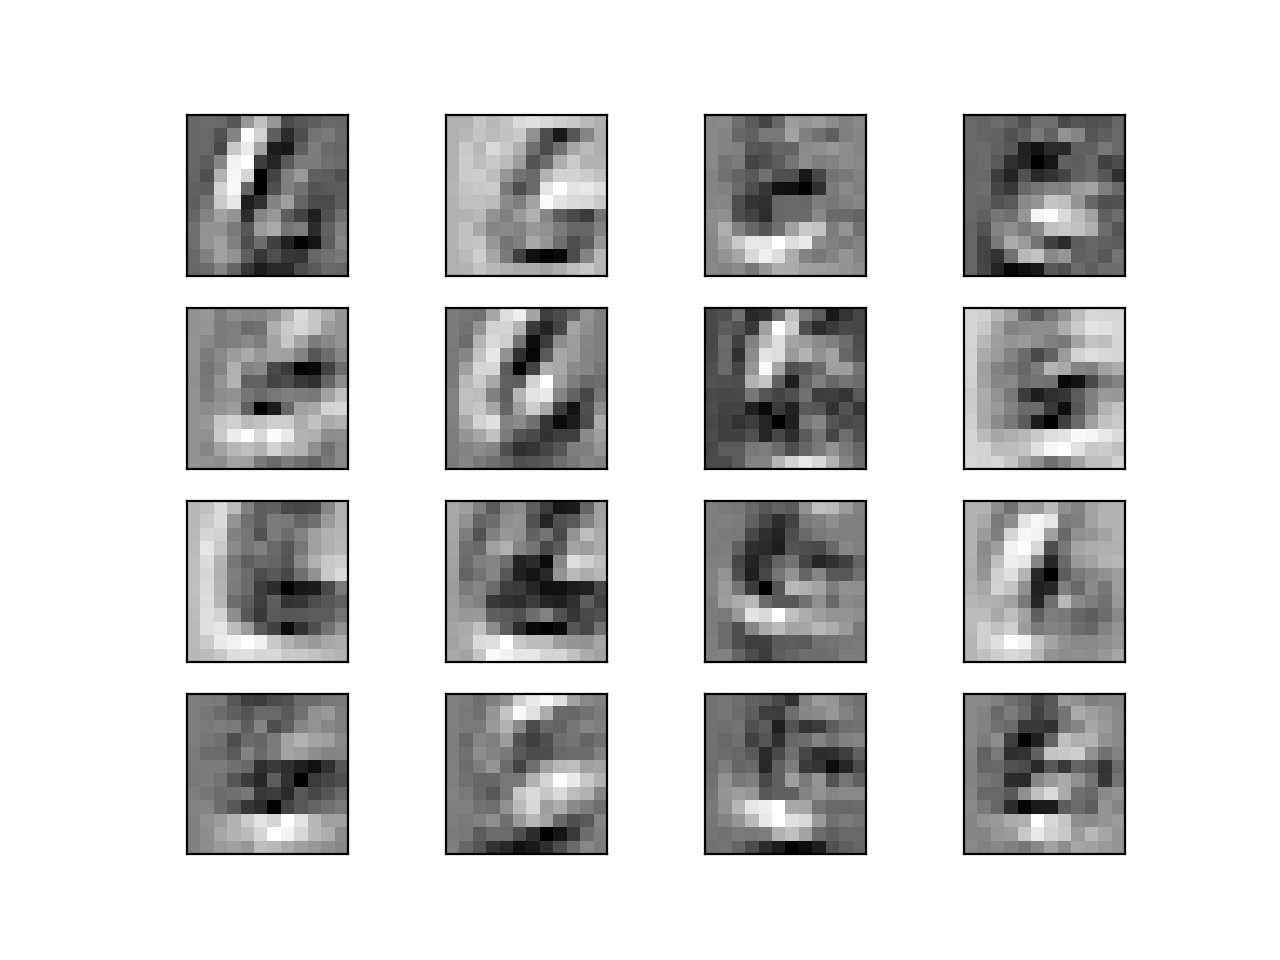
\includegraphics[scale=0.75]{resources/second_layer_gd_lenet.png}}
\caption{Mapy aktywacji dla 16 filtrów warstwy drugiej, przy użyciu przykładowej reprezentacji liczby 6.}
\label{fig:lenet5-mapy-aktywacji-l2}
\end{figure}

Uzyskane aktywacje wciąż przypominają oryginalną szóstkę, lecz tym razem, zgodnie z oczekiwaniami, cechy są bardziej zgeneralizowane.
Wyraźnie widać skupienie filtrów na dolnej ''pętli'' szóstki oraz na tym, by posiadała odpowiednie łuki na brzegach (wyraźnie zarysowany jest tam gradient, widoczny szczególnie na filtrach w ostatnim rzędzie).

Niestety sieć LeNet-5 jest na tyle płytka a zestaw odręcznie pisanych cyfr na tyle mało skomplikowany, że nie uda mi się przy ich pomocy wyekstrahować bardziej złożonych wzorów. W tym celu będę musiał posłużyć się bardziej złożonym modelem. Siecią VGG-16. 

\chapter{Wizualizacja przy pomocy warstw ukrytych sieci VGG-19}
\label{chap:vgg}
\section{Model sieci VGG-19}
\label{vgg-model}

Do bardziej złożonych wizualizacji posłużę się siecią VGG, której architekturę zaprezentowano po raz pierwszy w 2015 roku w publikacji autorstwa Karen Simonyan i 
Andrew Zisserman\cite{vggpaper}. W publikacji zaprezentowano kilka wariantów tej sieci. Ja z uwagi na większą liczbę warstw użyję wariantu VGG-19, którego schemat znajduje się na rysunku \ref{fig:vgg19-schemat}.

\begin{figure}[ht]
\centerline{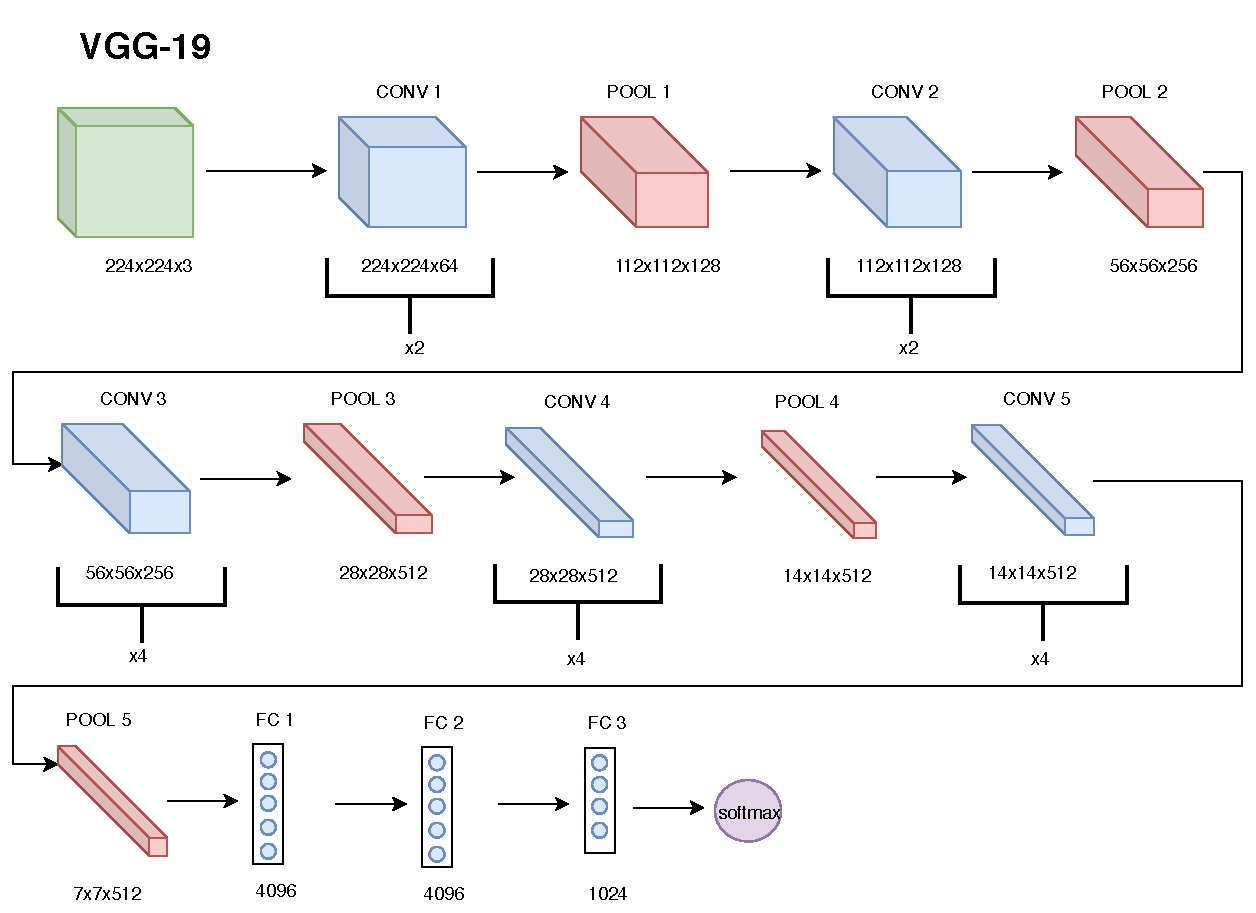
\includegraphics[scale=0.5]{resources/vgg/vgg.pdf}}
\caption{Schemat modelu sieci VGG-19.}
\label{fig:vgg19-schemat}
\end{figure}

Dopełnienie w przypadku warstw konwolucyjnych wynosi \(p=1\) przy skoku \(s=1\) co sprawia, że warstwy konwolucyjne mogą być ze sobą łączone w łańcuchy niezmieniające wymiarów tensora. W przypadku warstw \textit{poolingowych} \(p=1\) przy skoku \(s=2\) tym samym, dzielą one dwa pierwsze wymiary przez pół. Sumarycznie daje to 16 warstw możliwych do wykorzystania w wizualizacjach.

\subsection{Wizualizacja poprzez rekonstrukcję obrazu przy pomocy maksymalizacji aktywacji neuronu}
\label{vgg-mean-activation}

Z racji swoich rozmiarów, trening sieci VGG zajmuje dni, nawet przy pomocy GPU. Użyję więc wcześniej wytrenowanej sieci dostępnej bezpośrednio w Kerasie.

\begin{lstlisting}[language=Python, caption={Wczytywanie wag VGG-19 w Keras.}, label={lst:vggkeras}, captionpos=b]
from keras.applications import VGG19
model = VGG19(include_top=False, weights='imagenet')
\end{lstlisting}

Zastosowane opcje to przede wszystkim zestaw danych na, których była trenowana sieć, w tym wypadku zbiór ImageNet\cite{imagenet}, oraz wyłączenie z ładowanego modelu warstw gęstch. Ta ostatnia opcja pozwoli na rekonstukcję obrazu o dowolnej liczbie pikseli (zamiast standardowego dla architektury VGG 224\(\times\)224 pikseli).

Mając załadowany model wraz z wytrenowanymi wagami, wybieram poszczególne filtry z kolejnych warstw konwolucyjnych. Następnie, generuję losowy (wartość pikseli losowana jest z rozkładu jednorodnego) obrazek o niskiej rozdzielczości, początkowo szary obraz zaburzam nieznacznie różnymi kolorami i wyliczam aktywacje wybranej wcześniej warstwy.
Przykładowy obraz wejściowy przedstawia rysunek \ref{fig:obrazwe}

\begin{figure}[ht]
\centerline{
\includegraphics[scale=1]{resources/cnn/obrazwe.png}}
\caption{Obraz wejściowy dla skryptu maksymalizującego medianę warstwy.}
\label{fig:obrazwe}
\end{figure}

Medianę z tych aktywacji traktuję jako wartość mojej funkcji kosztu i modyfikuję wylosowany uprzednio obrazek w celu jej maksymalizacji.

Maksymalizacja aktywacji jest możliwa poprzez wywołanie metody o nazwie \textit{gradients} z biblioteki Keras. Wykorzystując ją można przy pomocy tensora wejściowego, w tym wypadku zdjęcia, oraz funkcji kosztu (zdefiniowanej powyżej) uzyskać gradient funkcji kosztu dla danych z tensora.
Następnie, moim celem będzie wykonać operację odwrotną niż w podczas treningu sieci -- maksymalizację funkcji kosztu. Uzyskany gradient wykorzystywany jest do przekształcania obrazu.

Modyfikacja obrazu polega na dodaniu odpowiednio znormalizowanego gradientu do wartości poszczególnych pikseli. Cały proces treningu składa się z kilkukrotnego skalowania obrazu do wyższych ,,rozdzielczości'' i ponawiania procesu optymalizacji. 

Skalowanie jest konieczne, ponieważ struktury generowane tą metodą charakteryzują się wysoką częstotliwością (są małe i powtarzalne). Uprzednie wygenerowanie fragmentu wzoru w niskiej rozdzielczości i skalowanie, sprawia, że często wzór jest niejako ,,dobudowywany'' zamiast powtarzany, przez co jest większy -- co czasem daje lepsze zrozumienie na co patrzymy, choć nie jest to niestety reguła.

\begin{lstlisting}[language=Python, caption={Wizualizowanie poprzez maksymalizację mediany wybranej warstwy.}, label={lst:vggmeantraining}, captionpos=b]
output = layers_by_name[layer_name].output
loss = K.mean(output[:, :, :, filter_index])
gradients = K.gradients(loss, input_tensor)[0]
img = generate_grascale_img();
for interpolation_step in image_resize_steps:
    for i in range(EPOCHS_NUMBER):
        loss_val, gradients_val = step([img])
        img += gradients_val 
    resize_img(img);
\end{lstlisting}

Listing \ref{lst:vggmeantraining} zawiera wysokopoziomowy zarys tego, w jaki sposób działa skrypt generujący poniższe wizualizacje. Wszystkie szczegóły implementacyjne, takie jak normalizacja gradientu czy konwersja obrazu z postaci nadającej się do treningu na postać zdatną do wyświetlenia zostały pominięte.

Zgodnie z oczekiwaniami, złożoność uzyskanych wizualizacji rośnie wraz numerem warstwy, na podstawie której je uzyskano. Uzyskane obrazy nie prezentują żadnej ze znanych mi klas na których trenowano tę konkretną instancję VGG19, a raczej ,,teksturę'' obserwowanego przedmiotu.

Pierwsze warstwy nie są zbytnio bogate w informacje. Kodują podstawowe informacje o kolorze, nie posiadając zbyt wiele informacji o strukturze klasyfikowanego przedmiotu. Choć i już tu trafiają się ciekawe wizualizacje jak np. filtru 5 warstwy conv1 bloku 1 - przypominającej trochę księżyc. 

U części z tych wizualizacji (szczególnie na dalszych początkowych warstwch) można zaobserwować struktury przypominające korę drzew. Kolejne wizualizacje robią się bardziej kolorowe i przechodzą w bardziej abstrakcyjne wzory, które wciąż możnaby wziąć za tkaninę czy chmurę. Niestety uchwycone zależności na warstwach głębokich, choć fascynujące, są poza moimi możliwościami interpretacji.

Choć przytoczony w pracy zestaw wizualizacji nie posiada dużej ich reprezentacji, podczas tworzenia wizualizacji natknąłem się na wiele podobnych do siebie struktur, nieznacznie tylko obróconych o jakiś kąt. Za przykład może posłużyć wizualizacja z warstw conv5 bloku 1, filtry 30 i 3 na rysunku \ref{mean-vgg-vis-c5bx}.

Biorąc pod uwagę to, że w sieciach CNN filtry aplikowane są cały czas w taki sam sposób, czyli od lewej do prawej, z góry na dół; a przedmioty występujące w danych wejściowych często występują w różnych położeniach nie wydaje się być zaskakujące, że istnieje potrzeba stosowania takich samych filtrów o różnych rotacjach. 
Jest to zaskakująco analogiczna sytuacja jak w klasycznej analizie obrazu, gdzie stosowane filtry do wykrywania krawędzi pionowych i poziomych są takimi samymi, po uprzedniej operacji transponowania, macierzami.
Pozostawia to pole do poprawy działania takich sieci. Odpowiednie kadrowanie, rotacja danych wejściowych lub jakakolwiek forma adaptacyjnej aplikacji fitrów mogłaby sprawić, że trening tych samych, obróconych filtrów byłby zbędny co w rezultacie sprawiłoby, że nie potrzeba byłoby ich tak dużo, co mogłoby skrócić trening sieci przy braku negatywnego wpływu na sprawność predykcji.

Rysunki \ref{mean-vgg-vis-c1bx}, \ref{mean-vgg-vis-c2bx}, \ref{mean-vgg-vis-c3bx}, \ref{mean-vgg-vis-c4bx} i \ref{mean-vgg-vis-c5bx} przedstawiają uzyskane wizualizacje przy pomocy wyżej opisanego procesu.
\begin{figure}
\subfloat[Wizualizacja filtra nr 5 bloku 1]{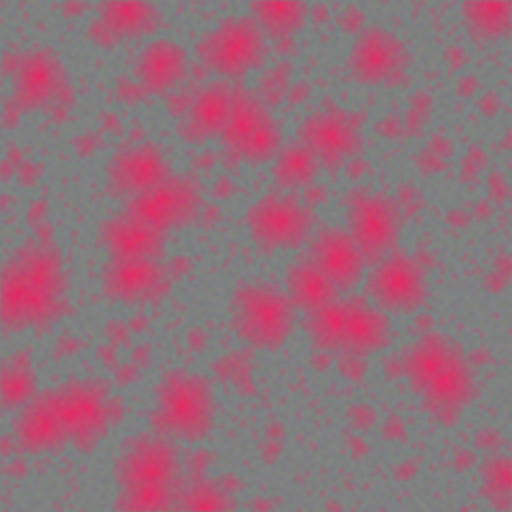
\includegraphics[width = 2in]{resources/vgg_mean_res/block1_conv1_5.png}} 
~
\subfloat[Wizualizacja filtra nr 15 bloku 1]{
\includegraphics[width = 2in]{resources/vgg_mean_res/block1_conv1_15.png}} 
~
\subfloat[Wizualizacja filtra nr 9 bloku 1]{
\includegraphics[width = 2in]{resources/vgg_mean_res/block1_conv1_9.png}} 
\\
\subfloat[Wizualizacja filtra nr 50 bloku 2]{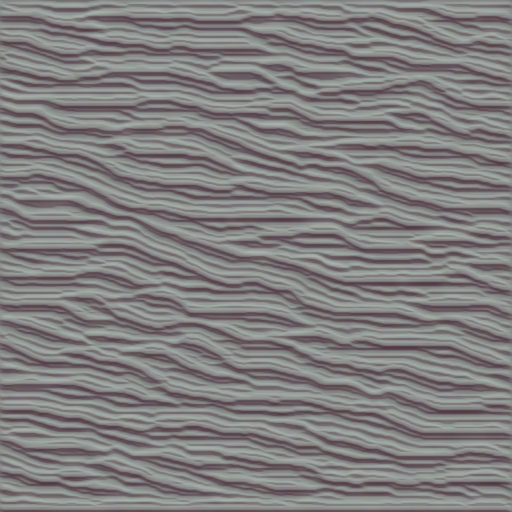
\includegraphics[width = 2in]{resources/vgg_mean_res/block1_conv2_50.png}} 
~
\subfloat[Wizualizacja filtra nr 32 bloku 2]{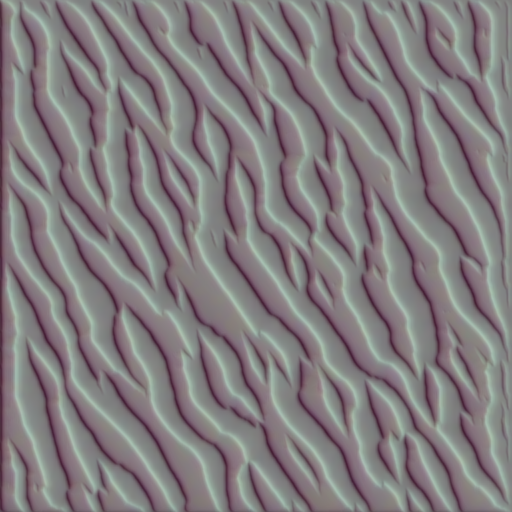
\includegraphics[width = 2in]{resources/vgg_mean_res/block1_conv2_32.png}} 
~
\subfloat[Wizualizacja filtra nr 33 bloku 2]{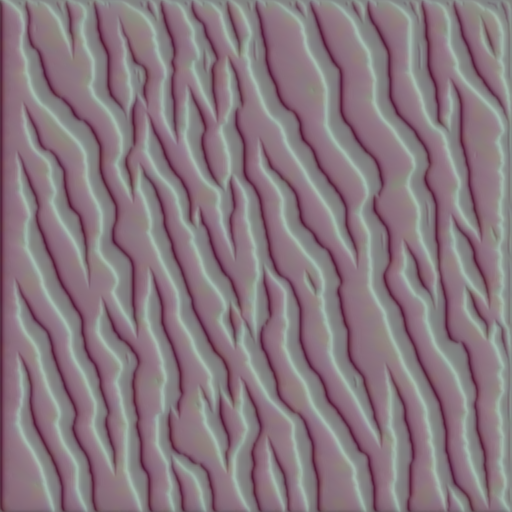
\includegraphics[width = 2in]{resources/vgg_mean_res/block1_conv2_33.png}} 
\\
\subfloat[Wizualizacja filtra nr 59 bloku 2]{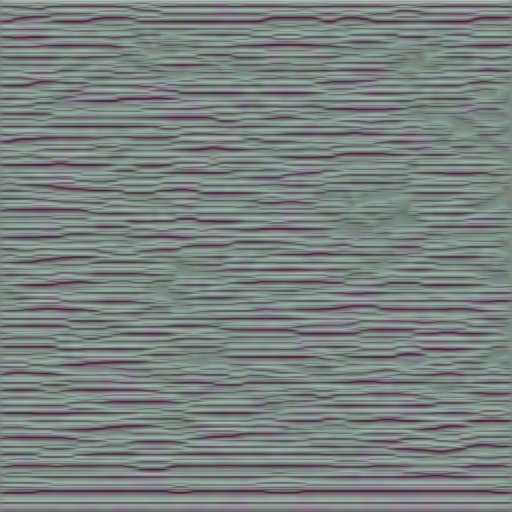
\includegraphics[width = 2in]{resources/vgg_mean_res/block1_conv2_59.png}} 
~
\subfloat[Wizualizacja filtra nr 60 bloku 2]{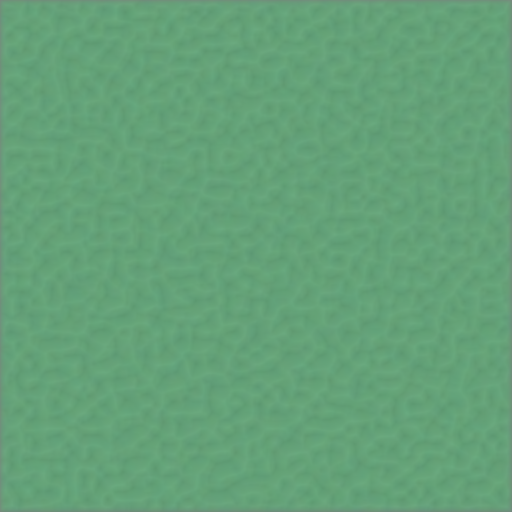
\includegraphics[width = 2in]{resources/vgg_mean_res/block1_conv2_60.png}} 
~
\subfloat[Wizualizacja filtra nr 61 bloku 2]{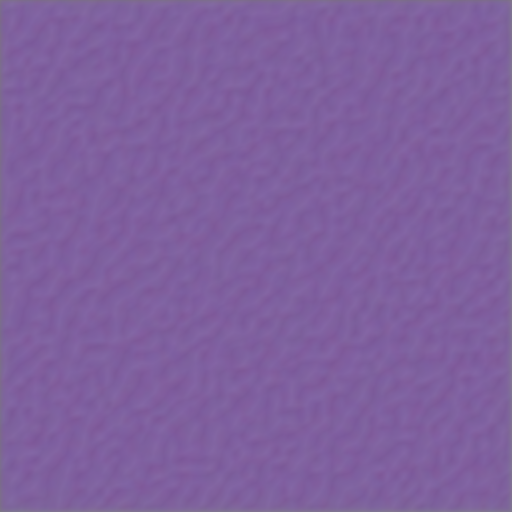
\includegraphics[width = 2in]{resources/vgg_mean_res/block1_conv2_61.png}} 
\caption{Wybrane wizualizacje warstwy sieci VGG-19 oznaczonej na rysunku \ref{vgg-model} jako conv1}
\label{mean-vgg-vis-c1bx}
\end{figure}

\begin{figure}
\subfloat[Wizualizacja filtra nr 120 bloku 2]{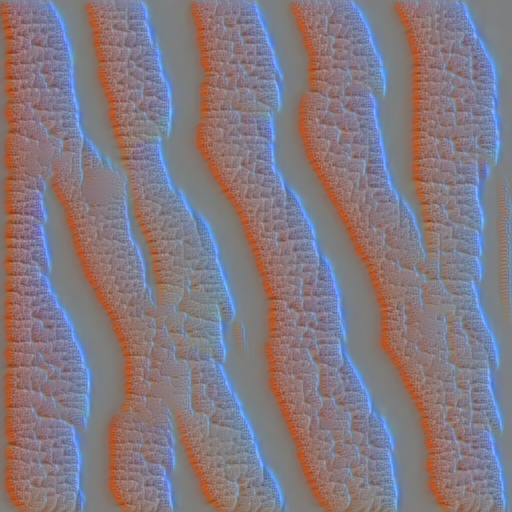
\includegraphics[width = 2in]{resources/vgg_mean_res/block2_conv2_120.png}} 
~
\subfloat[Wizualizacja filtra nr 60 bloku 2]{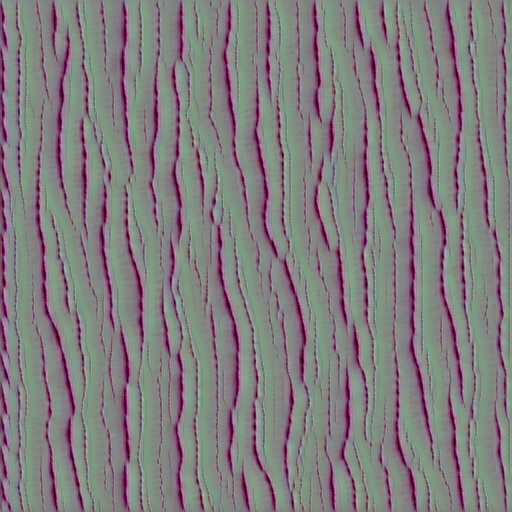
\includegraphics[width = 2in]{resources/vgg_mean_res/block2_conv2_60.png}} 
~
\subfloat[Wizualizacja filtra nr 80 bloku 2]{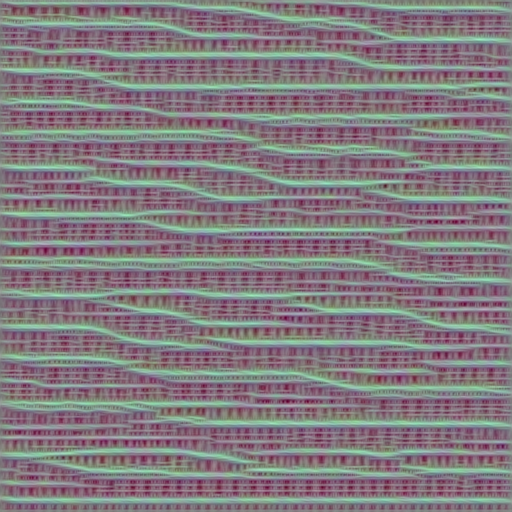
\includegraphics[width = 2in]{resources/vgg_mean_res/block2_conv2_80.png}} 
\\
\subfloat[Wizualizacja filtra nr 33 bloku 1]{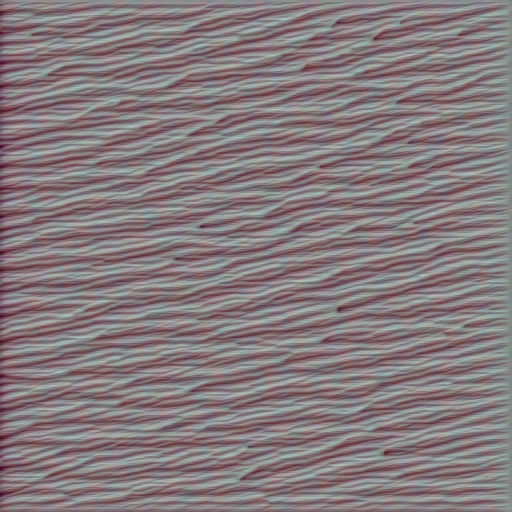
\includegraphics[width = 2in]{resources/vgg_mean_res/block2_conv1_33.png}} 
~
\subfloat[Wizualizacja filtra nr 32 bloku 1]{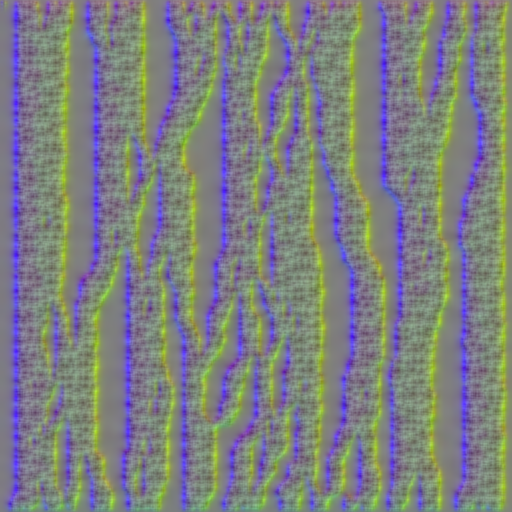
\includegraphics[width = 2in]{resources/vgg_mean_res/block2_conv1_32.png}} 
~
\subfloat[Wizualizacja filtra nr 19 bloku 1]{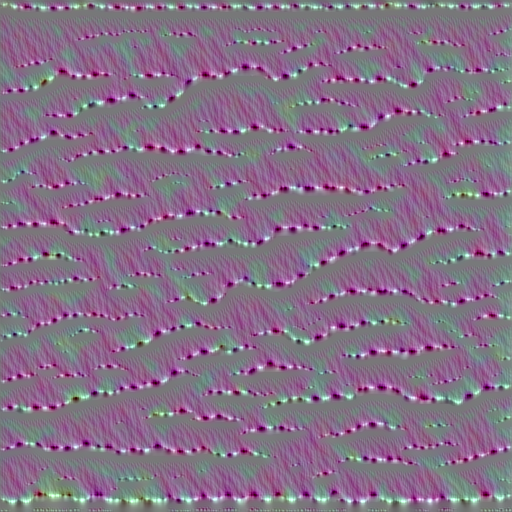
\includegraphics[width = 2in]{resources/vgg_mean_res/block2_conv1_19.png}} 
\\
\subfloat[Wizualizacja filtra nr 63 bloku 2]{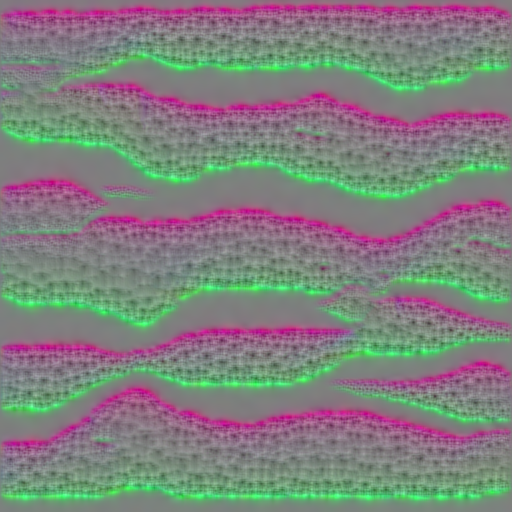
\includegraphics[width = 2in]{resources/vgg_mean_res/block2_conv2_63.png}} 
~
\subfloat[Wizualizacja filtra nr 64 bloku 2]{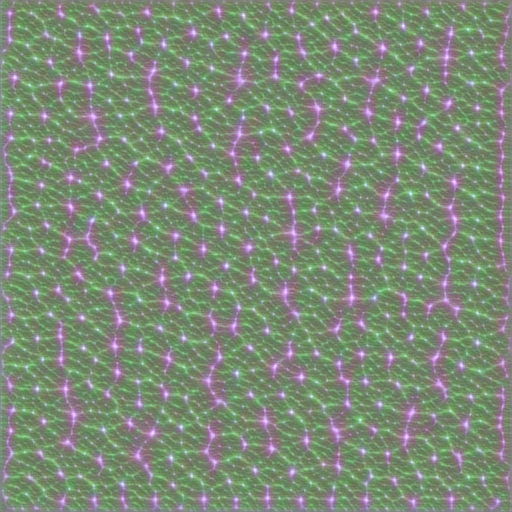
\includegraphics[width = 2in]{resources/vgg_mean_res/block2_conv2_64.png}} 
~
\subfloat[Wizualizacja filtra nr 65 bloku 2]{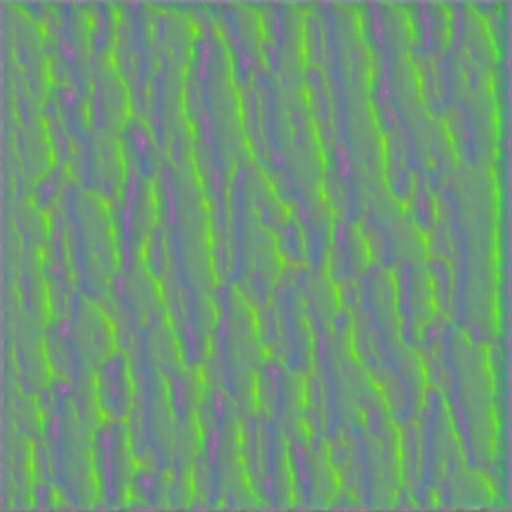
\includegraphics[width = 2in]{resources/vgg_mean_res/block2_conv2_65.png}} 

\caption{Wybrane wizualizacje warstwy sieci VGG-19 oznaczonej na rysunku \ref{vgg-model} jako conv2}
\label{mean-vgg-vis-c2bx}
\end{figure}

\begin{figure}
\subfloat[Wizualizacja filtra nr 128 bloku 4]{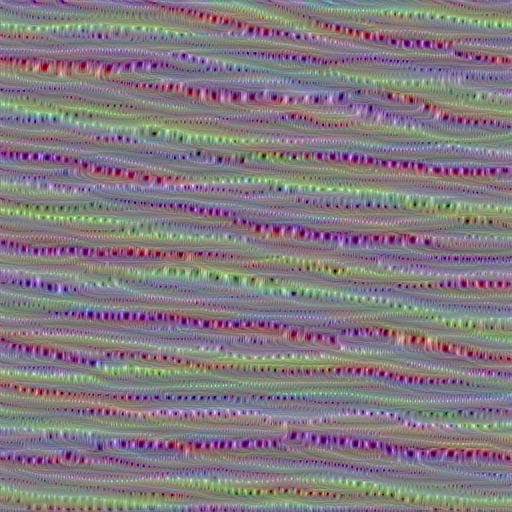
\includegraphics[width = 2in]{resources/vgg_mean_res/block3_conv4_128.png}} 
~
\subfloat[Wizualizacja filtra nr 17 bloku 4]{
\includegraphics[width = 2in]{resources/vgg_mean_res/block3_conv4_17.png}} 
~
\subfloat[Wizualizacja filtra nr 9 bloku 2]{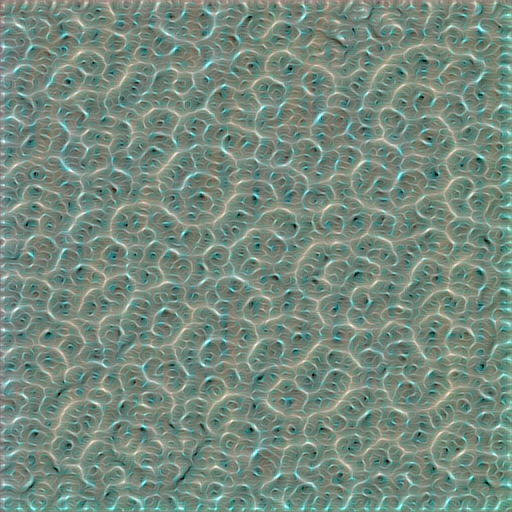
\includegraphics[width = 2in]{resources/vgg_mean_res/block3_conv2_9.png}} 
\\
\subfloat[Wizualizacja filtra nr 34 bloku 3]{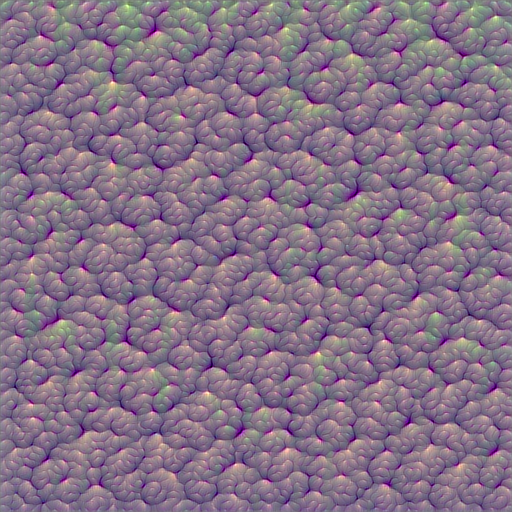
\includegraphics[width = 2in]{resources/vgg_mean_res/block3_conv3_34.png}} 
~
\subfloat[Wizualizacja filtra nr 15 bloku 1]{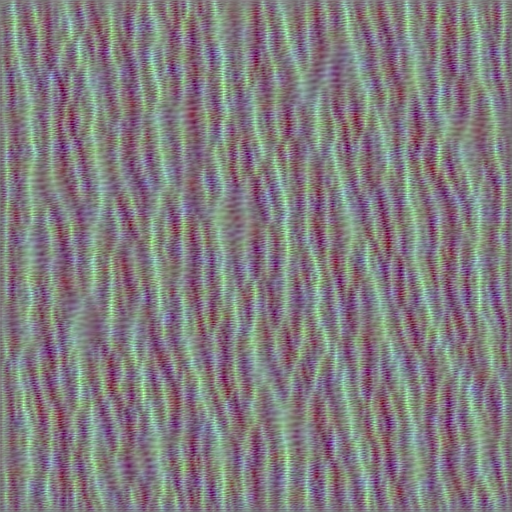
\includegraphics[width = 2in]{resources/vgg_mean_res/block3_conv1_15.png}} 
~
\subfloat[Wizualizacja filtra nr 32 bloku 3]{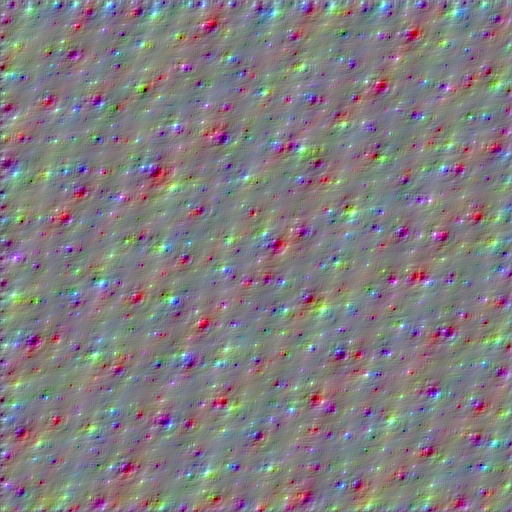
\includegraphics[width = 2in]{resources/vgg_mean_res/block3_conv3_32.png}} 
\\
\subfloat[Wizualizacja filtra nr 254 bloku 4]{
\includegraphics[width = 2in]{resources/vgg_mean_res/block3_conv4_254.png}} 
~
\subfloat[Wizualizacja filtra nr 32 bloku 4]{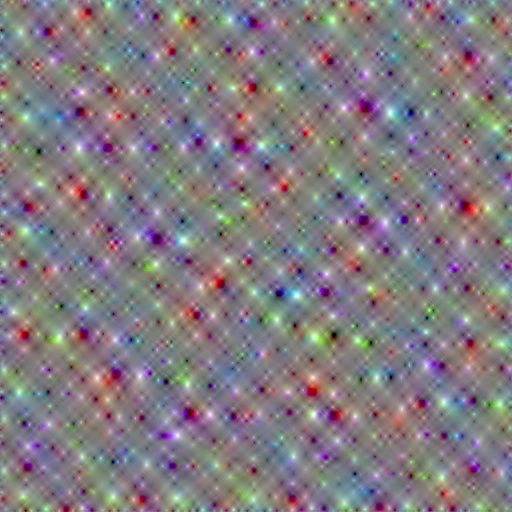
\includegraphics[width = 2in]{resources/vgg_mean_res/block3_conv4_32.png}} 
~
\subfloat[Wizualizacja filtra nr 33 bloku 4]{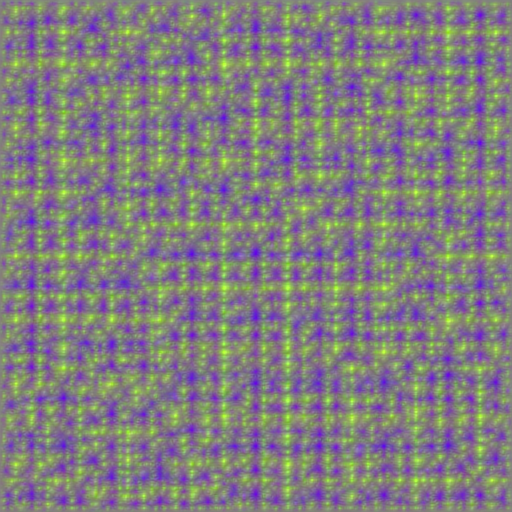
\includegraphics[width = 2in]{resources/vgg_mean_res/block3_conv1_59.png}} 

\caption{Wybrane wizualizacje warstwy sieci VGG-19 oznaczonej na rysunku \ref{vgg-model} jako conv3}
\label{mean-vgg-vis-c3bx}
\end{figure}

\begin{figure}
\subfloat[Wizualizacja filtra nr 128 bloku 4]{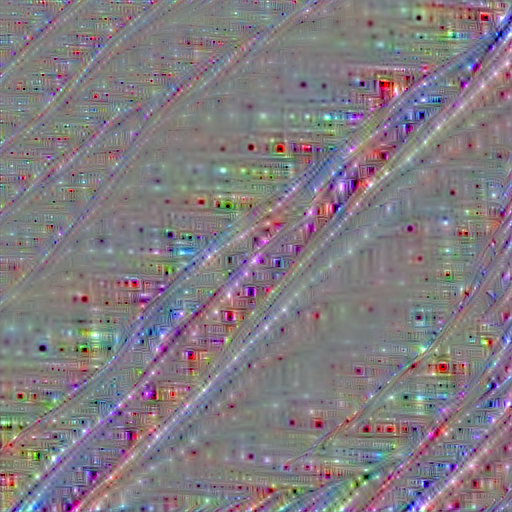
\includegraphics[width = 2in]{resources/vgg_mean_res/block4_conv4_128.png}} 
~
\subfloat[Wizualizacja filtra nr 17 bloku 4]{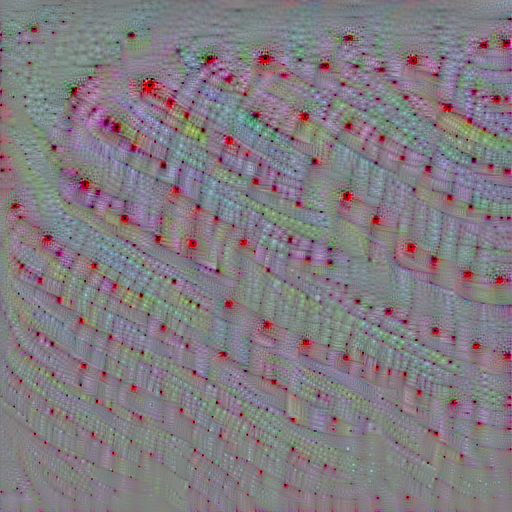
\includegraphics[width = 2in]{resources/vgg_mean_res/block4_conv4_17.png}} 
~
\subfloat[Wizualizacja filtra nr 32 bloku 4]{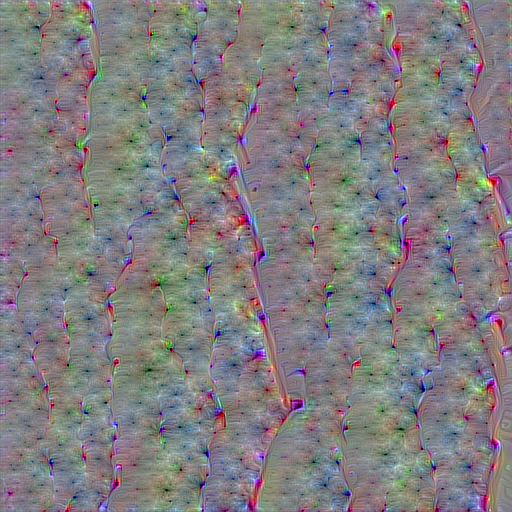
\includegraphics[width = 2in]{resources/vgg_mean_res/block4_conv4_32.png}} 
\\
\subfloat[Wizualizacja filtra nr 10 bloku 1]{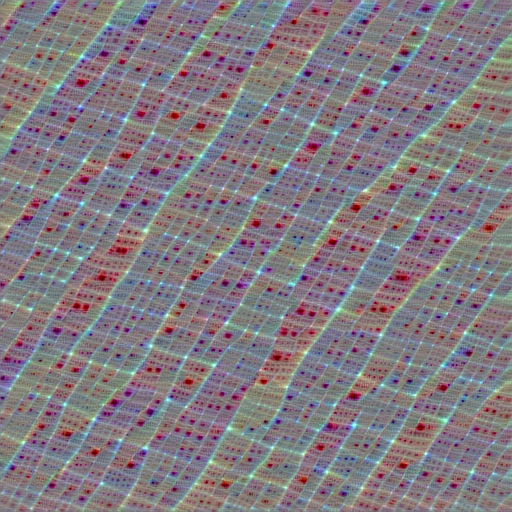
\includegraphics[width = 2in]{resources/vgg_mean_res/block4_conv1_10.png}} 
~
\subfloat[Wizualizacja filtra nr 11 bloku 2]{\includegraphics[width = 2in]{resources/vgg_mean_res/block4_conv2_11.png}} 
~
\subfloat[Wizualizacja filtra nr 15 bloku 3]{\includegraphics[width = 2in]{resources/vgg_mean_res/block4_conv3_15.png}} 
\\
\subfloat[Wizualizacja filtra nr 59 bloku 1]{\includegraphics[width = 2in]{resources/vgg_mean_res/block4_conv1_59.png}} 
~
\subfloat[Wizualizacja filtra nr 64 bloku 2]{\includegraphics[width = 2in]{resources/vgg_mean_res/block4_conv2_64.png}} 
~
\subfloat[Wizualizacja filtra nr 65 bloku 3]{\includegraphics[width = 2in]{resources/vgg_mean_res/block4_conv3_65.png}} 

\caption{Wybrane wizualizacje początkowej warstwy sieci VGG-19 (oznaczonej na rysunku \ref{vgg-model} jako conv4)}
\label{mean-vgg-vis-c4bx}
\end{figure}

\begin{figure}
\subfloat[Wizualizacja filtra nr 120 bloku 1]{\includegraphics[width = 2in]{resources/vgg_mean_res/block5_conv1_120.png}} 
~
\subfloat[Wizualizacja filtra nr 3 bloku 1]{\includegraphics[width = 2in]{resources/vgg_mean_res/block5_conv1_3.png}} 
~
\subfloat[Wizualizacja filtra nr 30 bloku 1]{\includegraphics[width = 2in]{resources/vgg_mean_res/block5_conv1_30.png}} 
\\
\subfloat[Wizualizacja filtra nr 60 bloku 1]{\includegraphics[width = 2in]{resources/vgg_mean_res/block5_conv1_60.png}} 
~
\subfloat[Wizualizacja filtra nr 60 bloku 2]{\includegraphics[width = 2in]{resources/vgg_mean_res/block5_conv2_60.png}} 
~
\subfloat[Wizualizacja filtra nr 63 bloku 4]{\includegraphics[width = 2in]{resources/vgg_mean_res/block5_conv4_63.png}} 
\\
\subfloat[Wizualizacja filtra nr 63 bloku 2]{\includegraphics[width = 2in]{resources/vgg_mean_res/block5_conv2_63.png}} 
~
\subfloat[Wizualizacja filtra nr 90 bloku 1]{\includegraphics[width = 2in]{resources/vgg_mean_res/block5_conv1_90.png}} 
~
\subfloat[Wizualizacja filtra nr 65 bloku 4]{\includegraphics[width = 2in]{resources/vgg_mean_res/block5_conv4_65.png}} 
\caption{Wybrane wizualizacje warstwy sieci VGG-19 oznaczonej na rysunku \ref{vgg-model} jako conv5}
\label{mean-vgg-vis-c5bx}
\end{figure}

\subsection{Wizualizacja maksymalnej aktywacji danej klasy}
\label{vgg-class-visualisation}

VGG19 w inny od człowieka sposób uchwyca to, czym jest dany na obrazie przedmiot. By zwizualizować w jaki sposób sieć odróżnia poszczególne klasy, można posłużyć się analogicznym sposóbem postępowania jak z podrozdziału \ref{vgg-mean-activation}.
Jeżeli do modelu przywrócić warstwy gęste i próbować zmaksymalizować aktywację dla jednej z klas poprzez modyfikację obrazu wejściowego, powinienem otrzymać obraz, który sieć bezwątpliwie traktowałaby jako reprezentanta danej klasy.
Gdyby sieć miała w sobie zakodowaną informację o tym, co tak naprawdę jest na obrazie, powinienem otrzymać coś przynajmniej odlegle przypominającego oryginalną klasę.

Weźmy przykładowo klasę numer 319. W przypadku tego konkretnego modelu odpowiada ona klasie ważki. Przykładowego przedstawiciela tej klasy przedstawia rysunek \ref{fig:wazka-real}.

\begin{figure}[ht]
\centerline{\includegraphics[scale=0.8]{resources/vgg_mean_topincluded/dragonfly.jpeg}}
\caption{Przykładowe zdjęcie ważki.}
\label{fig:wazka-real}
\end{figure}

\begin{lstlisting}[language=Python, caption={Predykcja klasy zdjęcia ważki (rys. \ref{fig:wazka-real}.)}, label={lst:wazkaprediction}, captionpos=b]
img = image.load_img('resources/vgg_mean_topincluded/dragonfly.jpeg', target_size=(224, 224))
x = image.img_to_array(img)
x = np.expand_dims(x, axis=0)
x = preprocess_input(x)
preds = model.predict(x)
print('Predicted:', decode_predictions(preds, top=3)[0])
\end{lstlisting}

\begin{lstlisting}[language=Python, caption={Wynik skryptu z listingu \ref{lst:wazkaprediction}.}, label={lst:wazkapredictionresult}, captionpos=b]
[('n02268443', 'dragonfly', 0.96805733), ('n02268853', 'damselfly', 0.01810956), ('n02264363', 'lacewing', 0.012446008)]
\end{lstlisting}

Wynik skryptu z listungu \ref{lst:wazkaprediction} jest widoczny na listngu \ref{lst:wazkapredictionresult}.

Oznacza to, że sieć, którą dysponuję, jest przekonana, że w zaokrągleniu na 97\% mamy do czynienia z ważką. Dwie kolejne najbardziej prawdopodobne klasy przedstawiają inny rodzaj ważki -- ważkę równoskrzydłą i owada siatkoskrzydłego.

Wszystko wydaje się być w porządku, dopóki nie wygenerujemy obrazu na podstawie wyżej wymienionej klasy. Uprzednio modyfikując funkcję kosztu tak, by teraz zwracała wartość, jaką przypisuje klasie ważki softmax, możemy zmodyfikować szary szum tak, by maksymalizować (wg. sieci) prawdopodobieństwo tego, że na obrazie jest ważka. Tym razem nie skaluję obrazu podczas treningu i modyfikuję obraz \(224 \times 224\).

\begin{figure}[ht]
\centerline{\includegraphics[scale=0.8]{resources/vgg_mean_topincluded/dragonfly-fake.png}}
\caption{Ważka uzyskana w odwróconym procesie treningu.}
\label{fig:wazka-fake}
\end{figure}

Mimo krótkiego czasu treningu taki obraz jak na rysunku \ref{fig:wazka-fake}, klasyfikowany jest przez sieć VGG19 jako ważka z pewnością sięgającą 96\%. Podobny wynik uzyskałem na wszystkich testowanych przeze mnie klasach. VGG rozpoznaje przedmioty na podstawie prawdopodobieństwa wystąpienia pewnej kombinacji filtrów -- niestety samo nie nadaje się do generowania realistycznych obrazów danej klasy. 
By uzyskać obrazy zdolne do oszukania ludzkiej percepcji należy posłużyć się architekturą typu GAN (\textit{ang. Generative Adversarial Networks}).

Niezwykle zajmującym tematem wydaje się być próba wprowadzenia uzyskanych wizualizacji do sieci VGG i uzyskanie odpowiedzi samej sieci, co jest na danym obrazie. 
Zmuszony jednak jestem zostawić temat wizualizacji uzyskanych za pomocą maksymalizacji aktywacji warstwy na rzecz innego zajmującego tematu -- neuronowego transferu stylu.

\section{\textit{Neural Style Transfer} przy pomocy sieci VGG}
\label{vgg-nst}
\textit{Neural Style Transfer} został pierwszy raz zaprezentowany w pracy autorstwa Leon A. Gatys, Alexander S. Ecker, Matthias Bethge \cite{nstpaper}.
Jest to technika mająca na celu uzyskanie obrazu \(G\) w stylu obrazu \(S\), przy pomocy obrazu bazowego \(B\) (patrz rys. \ref{neural-style-transfer-BSG}).

Jej oryginalni autorzy sami podają kluczową obserwację, umożliwiającą mieszanie obrazu. Jest to spostrzeżenie, że możliwe jest odesparowanie stylu i treści zakodowanych w aktywacjach sieci VGG.

Wszystkie wykorzystane wzory w tym podrozdziale pochodzą z publikacji \textit{A Neural Algorithm of Artistic Style} \cite{nstpaper}.

Załóżmy, że chcemy za pomocą wybranej warstwy konwolucyjnej sieci VGG odzwierciedlić treść obrazu \(C\) na obrazie \(G\). Mamy do wyboru warstwy oznaczone conv1...5.
Gdy wybierzemy jedną warstwę i wykonamy dla obrazów \(C\) i \(G\) kroki propagacji w przód otrzymamy mapy aktywacji \(a_{C}\) i \(a_{G}\). Korzystając z nich, można zdefiniować
funkcję kosztu: \[J_{c}^{[l]}(C, G) = \frac{1}{4 \times n_H \times n_W \times n_F} \sum{(a_{C} - a_{G})^{2}}, \tag{11}\]

gdzie:

\begin{itemize}
\item
    \(n_{W}\) -- szerokość filtra wybranej warstwy,
\item
    \(n_{H}\) -- wysokość filtra wybranej warstwy,
\item
    \(n_{F}\) -- liczba filtrów wybranej warstwy,
\item
    \(l\) -- numer zastosowanej warstwy.
\end{itemize}

Sumowanie odbywa się po wszystkich elementach mapy cech (uzyskana suma jest sumą aktywacji wszystkich warstw). 

Analogicznie można potraktować problem odzwierciedlenia stylu obrazu. Po wyborze warstwy uzyskujemy aktywację dla obrazów \(S\) i \(G\) oraz oznaczamy je kolejno \(a_{S}\) i \(a_{G}\). 
Następnie zwijamy tensory o wymiarach \(n_H \times n_W \times n_F\) w dwuwymiarowe macierze o wymiarach \((n_H + n_W) \times n_F\),  wyznaczamy macierze Grama tych macierzy i oznaczamy je jako 
\(G^{(S)}\) i \(G^{(G)}\). Wtedy można zdefiniować następującą funkcję kosztu stylu.

\[J_{s}^{[l]}(S,G) = \frac{1}{4 \times {n_F}^2 \times (n_H \times n_W)^2} \sum _{i=1}^{n_F}\sum_{j=1}^{n_F}(G^{(S)}_{ij} - G^{(G)}_{ij})^2 ,\tag{12}\]

Definiujemy zbiorczą funkcję kosztu jako:

\[J(G) = \alpha J_{c}(C,G) + \beta J_{s}(S,G), \tag{13}\]

gdzie:
\begin{itemize}
\item
    \(\alpha\) -- współczynnik kosztu treści,
\item
    \(\beta\) -- współczynnik kosztu stylu,
\end{itemize}

Sterując \(\alpha\) i \(\beta\) można wpływać na to jak bardzo obraz będzie wierny oryginałowi \textit{C} w stosunku do tego jak bardzo będzie namalowany w stylu \textit{S}. Używając tak zdefiniowanej funkcji kosztu dla jednej 
z warstw, można zapisać funkcję biorącą pod uwagę wyjście z kilku warstw konwolucyjnych jednocześnie: 

\[J_{s}(S,G) = \sum_{l} \lambda^{[l]} J^{[l]}_{s}(S,G), \tag{14}\]

gdzie \(\lambda^{[l]}\) jest współczynnikiem wykorzystania danej warstwy \(l\).

Przy pomocy tej funkcji można zastosować sposób działania znany z podrozdziału \ref{vgg-mean-activation}. Używając ją zamiast mediany aktywacji danej warstwy uzyskamy efekt widoczny na rysunku \ref{neural-style-transfer-BSG}. Szczegół implementacyjny: zaprezentowany obraz został wygenerowany przy pomocy skryptu napisanego w \textit{tensorflow}, a nie na podstawie modyfikacji opisanego wyżej skryptu.
Powód jest ściśle praktyczny dysponowałem już takim skryptem mojego autorstwa -- nie było praktyczne jednak wprowadzanie nowej biblioteki uczenia maszynowego, a jak było napisane wyżej, identyczne efekty można uzyskać przy pomocy Kerasa.

\begin{figure}
\subfloat[Obraz bazowy (B), autor zdjęcia: Grzegorz Rucki]{\includegraphics[width = 3in]{resources/nst/69850020.JPG}} 
~
\subfloat[Obraz stylu (S), ekpresjonistyczny - ''The keep''\cite{thekeep}]{\includegraphics[width = 2in]{resources/nst/the_keep_1958.jpg}} 
\\
\subfloat[Wygenerowany obraz (G)]{\includegraphics[width = 5in]{resources/nst/nst__at_iteration_9.png}} 
\caption{Transfer stylu na przykładzie zdjęcia z wakacji.}
\label{neural-style-transfer-BSG}
\end{figure}




%\bibliographystyle{alpha}
%\bibliography{bibliografia}
\printbibliography

\end{document}
